\documentclass[mathserif]{beamer}
\usepackage{beamerthemeshadow}
\usepackage{beamerthemesplit}
%\usetheme{shadow}
\usecolortheme{default}
\setbeamertemplate{footline}[frame number]
\useinnertheme[shadow=true]{rounded}
%\setbeamertemplate{footline}{\insertframenumber/\inserttotalframenumber}
%\useoutertheme{infolines}
%\setbeamertemplate{headline}{} % removes the headline that infolines inserts

%\usetheme{boxes}
%\usepackage{amsmass}
%\usepackage{amssymb,amsfonts,url}

\usepackage{algorithm}
\usepackage{algorithmic}

\usepackage{graphicx}
\graphicspath{{Problems/}}
\usepackage{caption}
\captionsetup[figure]{labelformat=simple}
\captionsetup[table]{labelformat=simple}


\usepackage{tikz}
\usetikzlibrary{shadows}
\usetikzlibrary{positioning}
\usepackage{verbatim}
\usepackage{pgfplots}
\usepackage{verbatim}
\usetikzlibrary{arrows,shapes}

\definecolor{darkblue}{rgb}{0.2,0.2,0.6}
\definecolor{darkred}{rgb}{0.6,0.1,0.1}
\definecolor{darkgreen}{rgb}{0.2,0.6,0.2}

\usetikzlibrary{shadings,shadows,shapes.arrows}

\usetikzlibrary{calc} 
\makeatletter 
\@namedef{color@3}{blue!20}
\@namedef{color@1}{green!70}   
%\@namedef{color@3}{yellow!50} 
\@namedef{color@2}{orange!90}  
%\@namedef{color@5}{magenta!70} 
%\@namedef{color@6}{yellow!70}    

\newcommand{\graphitemize}[2]{%
\begin{tikzpicture}[every node/.style={align=center}, scale=0.78]  
 \draw[fill=green!5, fill opacity=0.1, green, inner sep=0.05cm, outer sep=0.05cm] (5,0) arc(0:360:5);
 % \draw[fill=white,draw=white, fill opacity=0.1, white, inner sep=0.05cm, outer sep=0.05cm] (4,0) arc(0:360:4);
%  \shade[ball color=gray!10!] (0,0) coordinate(Hp) circle (.9);
  \node[shape=circle,  minimum size=1.1cm,fill=red!60,font=\Large,outer sep =.15cm,inner sep=.2cm,drop  shadow={ashadow, color=red!60!black}](ce){#1};  
   % \shade[ball color=blue!20!] (0,0) coordinate($Algorithm$) circle (1.5cm);

\foreach \gritem [count=\xi] in {#2}  {\global\let\maxgritem\xi}  
\foreach \gritem [count=\xi] in {#2}
{% 
\pgfmathtruncatemacro{\angle}{90+360/\maxgritem*\xi}
\edef\col{\@nameuse{color@\xi}}
\node[shape=circle,
     ultra thick,
     draw=white,
     fill opacity=1,
     drop  shadow={ashadow, color=blue!60},
     fill=\col,outer sep=0.25cm,        
     minimum size=2cm] (satellite-\xi) at (\angle:5cm) {\gritem };
     \draw[line width=0.25cm,-latex, \col] (ce) -- (satellite-\xi);
     }%
% \draw[violet, fill=violet!10] (4,0) arc(0:360:4);
\end{tikzpicture}  
}%



\newcommand*{\tikzarrow}[2]{%
  \tikz[
    baseline=(A.base),             % Set baseline to the baseline of node content
    font=\footnotesize\sffamily    % Set fontsize of the node content
  ]
  \node[
    single arrow,                  % Shape of the node
    single arrow head extend=2pt,  % Actual width of arrow head
    draw,                          % Draw the node shape
    inner sep=2pt,                 % Separation between node content and node shape
    top color=white,               % Shading color on top of node
    bottom color=#1,               % Shading color on bottom of node
    drop shadow                    % Draw a shadow
  ] (A) {#2};%
}


\def\arrow{
  (10.05:1.1) -- (6.05:1) arc (6.05:120:1) [rounded corners=0.5] --
  (120:0.9) [rounded corners=1] -- (130:1.1) [rounded corners=0.5] --
  (120:1.3) [sharp corners] -- (120:1.2) arc (120:5.25:1.2)
  [rounded corners=1] -- (10.05:1.1) -- (6.05:1) -- cycle
}

\tikzset{
  ashadow/.style={opacity=.25, shadow xshift=0.07, shadow yshift=-0.07},
}

\def\arrows[#1]{         
  \begin{scope}[scale=#1]
    \draw[color=darkred, drop  shadow={ashadow, color=red!60!black}] \arrow;

    \draw[color=darkgreen, bottom color=green!90!black, top color=green!60,   drop shadow={ashadow, color=green!60!black}] [rotate=120] \arrow;

    \draw[color=darkblue, right color=blue, left color=blue!60,   drop shadow={ashadow, color=blue!60!black}] [rotate=240] \arrow;

    % to hide the green shadow
    \draw[color=darkred, left color=red, right color=red!60] \arrow;
  \end{scope}
}
\tikzstyle{vertex}=[circle,fill=black!25,draw,minimum size=20pt,inner sep=0pt]
\tikzstyle{middlevertex}=[circle,fill=black!25,draw,minimum size=15pt,inner sep=0pt]
\tikzstyle{smallvertex}=[circle,fill=black!25,draw,minimum size=10pt,inner sep=0pt]
\tikzstyle{tinyvertex}=[circle,fill=black!25,draw,minimum size=6pt,inner sep=0pt]
\tikzstyle{selected vertex} = [vertex, draw,fill=red!24]
\tikzstyle{blue smallvertex} = [smallvertex, draw,fill=blue]
\tikzstyle{red smallvertex} = [smallvertex, draw,fill=red]
\tikzstyle{edge} = [draw,thick,->]
\tikzstyle{undirectededge} = [draw,thick]
\tikzstyle{weight} = [font=\small]
\tikzstyle{selected edge} = [draw,line width=3pt,-,red!50]
\tikzstyle{ignored edge} = [draw,line width=3pt,-,black!20]
\tikzstyle{squarednode}=[draw, fill=blue!20, thick, minimum size=5mm]
\tikzstyle{roundnode}=[circle, draw, fill=blue!20, thick, minimum size=5mm]



%\usepackage{CJK}
%\usepackage{pinyin}

%    \begin{figure}
%        \centering
%        \includegraphics[width=0.8\textwidth]{newGeneRep.eps}
%    \end{figure}

% \begin{figure}%
%   \begin{center}%
%     \begin{minipage}{0.70\textwidth}%
%      \includegraphics[width=1.0\textwidth]{comp25000.eps}%
%     \end{minipage}%
%     \begin{minipage}{0.30\textwidth}
%      \includegraphics[width=1.0\textwidth]{comparelabel.eps}%
%     \end{minipage}%
%   \end{center}
% \end{figure}

% \begin{table}
%   {\begin{tabular}{l|rrr}\line
%       & \multicolumn{3}{c}{Actual number of DCJ operations}\\
%       \# genes &\# genes $\times 1$&\# genes $\times 2$&\# genes  $\times 3$ \\
% \hline
%      (a)~25,000 & 0.5\% ~~&  0.9\% ~~& 1.7\%~~\\
%       (b)~10,000 & 0.8\%~~ &  1.4\% ~~& 2.7\%~~\\
%      (c)~ 1,000 & 2.7\%~~ & 4.7\%~~ & 14.7\%~~\\ \line
%     \end{tabular}} {}%
% \end{table}

% \begin{eqnarray}
% T(n) &=&  \sum_{i=1}^n C_i \\
%      &=&  \# PUSH + \#POP \\
%      &<& 2\times \#PUSH \\
%      &<& 2n \\
% \end{eqnarray}

% \[ 
% \begin{matrix}
% \begin{pmatrix}
% C_{11} & C_{12} \\ 
% C_{21} & C_{22} 
% \end{pmatrix}
% =
% \begin{pmatrix}
% A_{11} & A_{12} \\ 
% A_{21} & A_{22}  
% \end{pmatrix}
% 
% \begin{pmatrix}
% B_{11} & B_{12} \\ 
% B_{21} & B_{22}  
%  
% \end{pmatrix}
%     
%    \end{matrix}
% \]
% 
% 
% \begin{eqnarray}
%  C_{11} &=& (A_{11}\times B_{11}) + (A_{12} \times B_{21}) \\
% C_{12} &=& (A_{11}\times B_{12}) + (A_{12} \times B_{22}) \\
% C_{21} &=& (A_{21}\times B_{11}) + (A_{22} \times B_{21}) \\
% C_{22} &=& (A_{21}\times B_{12}) + (A_{22} \times B_{22}) 
% \end{eqnarray}


\title{CS711008Z  Algorithm Design and Analysis }
\subtitle{ Lecture 7. {\sc Union-Find} data structure 
\footnote{The slides were made  based on Chapter 5 of Algorithms by S. Dasgupta, C. H. Papadimitriou, and U. V. Vazirani, Data Structure by Ellis Horowitz, Hopcroft and Ullman 1973, and Tarjan 1975, et al.} 
}
\author{Dongbo Bu} 
\institute{ {\small Institute of Computing Technology \\ 
Chinese Academy of Sciences, Beijing, China}}

\date{}

\begin{document}
%\begin{CJK}{UTF8}{cyberbit}

\frame{\titlepage}

\frame{
\frametitle{Outline}
\begin{itemize}
\item Introduction to {\sc Union-Find} data structure 
\item Various implementations of {\sc Union-Find} data structure:
\begin{itemize}
\item Array: store ``set name" for each element separately. Easy to {\sc Find} set of any element, but hard to {\sc Union} two sets.  
\item Tree: each set is organized as a tree with root as ``set name". It is easy to {\sc Union} two sets, but hard to {\sc Find} set for an element.  
\item Link-by-rank: maintain a balanced-tree to limit tree depth to $O(\log n)$, making  {\sc Find} operations efficient.  
\item Link-by-rank and path compression: compress path when performing {\sc Find}, making subsequent {\sc Find} operations much quicker. 
\end{itemize}
\end{itemize}
}

\frame{
	\begin{block}{}
		{\sc Union-Find} data structure 
	\end{block}
}

\frame{
	\frametitle{ {\sc Union-Find}: motivation } 
	\begin{itemize}
		\item Motivation: Suppose we have a collection of \textcolor{red}{\bf disjoint sets}. The objective of {\sc Union-Find} is to keep track of elements by using the following operations: 
		\begin{itemize}
			\item {\sc MakeSet($x$)}: to create a new set $\{x\}$. 
			\item {\sc Find($x$)}: to find the set that contains the element $x$; 
			\item {\sc Union($x, y$)}: to union the two sets that contain elements $x$ and $y$, respectively. 
		\end{itemize}
		\item Analysis: total running time of a sequence of $m$ {\sc Find} and $n$ {\sc Union}. 
	\end{itemize}
} 


%\frame{
%	\frametitle{ Priority queue } 
%
%	\begin{itemize}
%		\item {\bf Priority queue}  is an \textcolor{red}{\bf abstract data type} similar to stack or queue, but each {\bf element} has a {\bf priority} associated with its {\bf name}. 
%		\item A min-oriented priority queue must  support the following core operations:  
%			\begin{enumerate}
%				\item $H$={\sc MakeHeap()}: to create a new heap $H$; 
%				\item {\sc Insert}$(H, x)$:  to insert into $H$ an element $x$ together with its priority
%				\item  {\sc ExtractMin}$(H)$:  to extract the element with the highest priority; 
%				\item {\sc DecreaseKey}$(H, x, k)$: to decrease the priority of element $x$; 
%%				\item {\sc FindMin}$(H)$: to find the element with the minimal priority; 
%%				\item {\sc IsEmpty}$(H)$: return whether the priority queue is empty or not; 
%%				\item {\sc Delete}$(H, x)$: to delete  element $x$ from $H$; 
%				\item {\sc Union}$(H_1, H_2)$: return a new heap containing all elements of heaps $H_1$ and $H_2$, and destroy the input heaps
%			\end{enumerate}
%	\end{itemize}
%}
\frame{
	\frametitle{{\sc Union-Find} is very useful} 
		\begin{itemize}
		\item {\sc Union-Find} has extensive applications, such as: 
			\begin{itemize}
				\item Network connectivity
				\item Kruskal's  MST algorithm
				\item Least common ancestor
				\item Games (Go)
				\item ......
			\end{itemize}
	\end{itemize}
}


\frame{
	\begin{block}{}
	An example: Kruskal's  MST algorithm
	\end{block}
}

\frame{
\frametitle{ Kruskal's algorithm [1956]  }

\begin{itemize}
\item Basic idea:  during the execution, $F$ is always an \textcolor{red}{\bf acyclic forest}, and the \textcolor{red}{\bf safe edge} added to $F$ is always a least-weight edge connecting two distinct components. 
\end{itemize}
\begin{figure}
     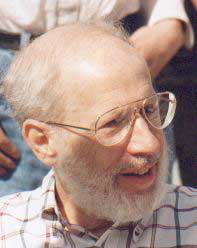
\includegraphics[width=1.5in]{Kruskal.png}
 \caption{ Joseph Kruskal} 
\end{figure}
} 

%
%
%
%\item 
%For graph $G$, we first construct its {\sc graphic matroid} $M_{G}=( S_G, {L} _G)$ as follows: 
%\begin{enumerate}
% \item {\sc Ground set: }  $S_G = E$, the set of edges; 
% \item {\sc Independent subsets:}  $A \in \mathcal{L}_G$ iff $A$ is acyclic. (Intuition: $A$ forms a forest, i.e.  a set of trees.)
% \item Weight: $w(e) = W_{max} - C(e)$, where $W_{max}$ is a large number to guarantee $w(e) > 0 $; 
%\end{enumerate}
%
%\item  
%Since $M_{G}$ is a matroid, the general {\sc Matroid\_Greedy} algorithm also applies: Kruskal's algorithm.
%\end{itemize}
%}

\frame{
\frametitle{ Kruskal's algorithm   [1956]}

{\sc MST-Kruskal}$( G, W )$
\begin{algorithmic}[1]
\STATE{ $F = \{ \}; $} 
\FORALL{ vertex $v \in V$ } 
\STATE{ {\sc MakeSet}$( v )$; }
\ENDFOR
\STATE\textcolor{red}{ sort the edges of $E$ into nondecreasing order by weight $W$; }
\FOR{ each edge $(u, v) \in E$ in the order } 
\IF { {\sc FindSet}$( u )$ $\neq$ {\sc FindSet}$( v )$ } 
\STATE $F = F \cup \{ ( u , v ) \};$ 
\STATE{{\sc Union} $( u, v )$; } 
\ENDIF
\ENDFOR
\end{algorithmic}

\begin{itemize}
\item 
Here,  {\sc Union-Find} structure is used to detect whether a set of edges form a cycle. 
\item Specifically, each set represents a connected component; thus, an edge connecting two nodes in the same set is ``unsafe'', as adding this edge will form a cycle. 
\end{itemize}

%(See extra slides for {\sc Union-Find} data structure, and a demo of Kruskal algorithm)
} 



\frame{
\frametitle{Kruskal's  MST algorithm: an example}

\begin{figure}

\begin{tikzpicture}[scale=0.9, auto,swap]

%problem 
     
    \foreach \pos/\name in {{(0,1)/s}, {(1.5,1)/a}, {(1.8, -0.8)/b}, {(0,-2.7)/c}, {(4.4 ,1)/d}, {(3.6,-2)/e}, {(5,-1.5)/f},{(6.5,-2.7)/t}}
        \node[middlevertex,fill=blue!20] (\name) at \pos {$\name$};
        
    \foreach \source/\dest/\weight in {s/a/9, s/b/14, s/c/15, a/d/24, b/d/18, b/e/30, c/e/20, d/e/2, e/f/11, e/t/16, f/t/6, d/t/19, c/t/44} 
                \draw[-, thick] (\source) -- node[above]{\small $\weight$} (\dest);
%initilization 
\pause
   \node[ultra thick, blue] at (3, 4) {Step 1}; 
  \node[ultra thick] at (3, 3) {Disjoint sets: $\{a\}, \{b\},\{c\},\{d\},\{e\},\{f\},\{s\},\{t\}$}; 
  \node[ultra thick] at (3, 3.5) {Edge weight: $\textcolor{green}{2}, 6, 9, 11, 14, 15, 16, 18, 19, 20, 24, 30, 44$}; 
%step 1
\pause
  \node[ ultra thick, green] at (8, 1) { {\sc Find}($d$) returns $\{d\}$}; 
  \node[ ultra thick, green] at (8, 0.5) { {\sc Find}($e$) returns $\{e\}$}; 
\pause
  \node[ ultra thick, green] at (8,  0.0) { {\sc Union}($d, e$)}; 
  
\pause  %clear and redraw
   \draw[fill=white,draw=white] (-2.7, 5) rectangle (10.5, -8); 
   \node[ultra thick, blue] at (3, 4) {Step 1}; 
  \node[ultra thick] at (3, 3) {Disjoint sets: $\{a\}, \{b\},\{c\},\{d, e\},\{f\},\{s\},\{t\}$}; 
  \node[ultra thick] at (3, 3.5) {Edge weight: $\textcolor{green}{2}, 6, 9, 11, 14, 15, 16, 18, 19, 20, 24, 30, 44$}; 
     
    \foreach \pos/\name in {{(0,1)/s}, {(1.5,1)/a}, {(1.8, -0.8)/b}, {(0,-2.7)/c}, {(4.4 ,1)/d}, {(3.6,-2)/e}, {(5,-1.5)/f},{(6.5,-2.7)/t}}
        \node[middlevertex,fill=blue!20] (\name) at \pos {$\name$};
        
    \foreach \source/\dest/\weight in {s/a/9, s/b/14, s/c/15, a/d/24, b/d/18, b/e/30, c/e/20, d/e/2, e/f/11, e/t/16, f/t/6, d/t/19, c/t/44} 
                \draw[-, thick] (\source) -- node[above]{\small $\weight$} (\dest);
    \foreach \source/\dest/\weight in { d/e/}   
  		\draw[-, ultra thick, red] (\source) -- node[above]{\small $\weight$} (\dest);

%step 2
\pause  %clear and redraw
   \draw[fill=white,draw=white] (-2.7, 5) rectangle (10.5, -8); 
   \node[ultra thick, blue] at (3, 4) {Step 2}; 
  \node[ultra thick] at (3, 3) {Disjoint sets: $\{a\}, \{b\},\{c\},\{d, e\},\{f\},  \{s\}, \{t\} $}; 
  \node[ultra thick] at (3, 3.5) {Edge weight: $2, \textcolor{green}{6}, 9, 11, 14, 15, 16, 18, 19, 20, 24, 30, 44$}; 
     
    \foreach \pos/\name in {{(0,1)/s}, {(1.5,1)/a}, {(1.8, -0.8)/b}, {(0,-2.7)/c}, {(4.4 ,1)/d}, {(3.6,-2)/e}, {(5,-1.5)/f},{(6.5,-2.7)/t}}
        \node[middlevertex,fill=blue!20] (\name) at \pos {$\name$};
        
    \foreach \source/\dest/\weight in {s/a/9, s/b/14, s/c/15, a/d/24, b/d/18, b/e/30, c/e/20, d/e/2, e/f/11, e/t/16, f/t/6, d/t/19, c/t/44} 
                \draw[-, thick] (\source) -- node[above]{\small $\weight$} (\dest);
    \foreach \source/\dest/\weight in { d/e/ }   
  		\draw[-, ultra thick, red] (\source) -- node[above]{\small $\weight$} (\dest);

\pause
  \node[ ultra thick, green] at (8, 1) { {\sc Find}($f$) returns $\{f\}$}; 
  \node[ ultra thick, green] at (8, 0.5) { {\sc Find}($t$) returns $\{t\}$}; 
\pause
  \node[ ultra thick, green] at (8,  0.0) { {\sc Union}($f, t$)}; 
  
\pause  %clear and redraw
   \draw[fill=white,draw=white] (-2.7, 5) rectangle (10.5, -8); 
   \node[ultra thick, blue] at (3, 4) {Step 2}; 
  \node[ultra thick] at (3, 3) {Disjoint sets: $\{a\}, \{b\},\{c\},\{d, e\},\{f, t\},\{s\} $}; 
  \node[ultra thick] at (3, 3.5) {Edge weight: $2, \textcolor{green}{6}, 9, 11, 14, 15, 16, 18, 19, 20, 24, 30, 44$}; 
     
    \foreach \pos/\name in {{(0,1)/s}, {(1.5,1)/a}, {(1.8, -0.8)/b}, {(0,-2.7)/c}, {(4.4 ,1)/d}, {(3.6,-2)/e}, {(5,-1.5)/f},{(6.5,-2.7)/t}}
        \node[middlevertex,fill=blue!20] (\name) at \pos {$\name$};
        
    \foreach \source/\dest/\weight in {s/a/9, s/b/14, s/c/15, a/d/24, b/d/18, b/e/30, c/e/20, d/e/2, e/f/11, e/t/16, f/t/6, d/t/19, c/t/44} 
                \draw[-, thick] (\source) -- node[above]{\small $\weight$} (\dest);
    \foreach \source/\dest/\weight in { d/e/, f/t/ }   
  		\draw[-, ultra thick, red] (\source) -- node[above]{\small $\weight$} (\dest);
  

%step 3
\pause  %clear and redraw
   \draw[fill=white,draw=white] (-2.7, 5) rectangle (10.5, -8); 
   \node[ultra thick, blue] at (3, 4) {Step 3}; 
  \node[ultra thick] at (3, 3) {Disjoint sets: $\{a\}, \{b\},\{c\},\{d, e\},\{f, t\},\{s\} $}; 
  \node[ultra thick] at (3, 3.5) {Edge weight: $2, 6, \textcolor{green}{9}, 11, 14, 15, 16, 18, 19, 20, 24, 30, 44$}; 
     
    \foreach \pos/\name in {{(0,1)/s}, {(1.5,1)/a}, {(1.8, -0.8)/b}, {(0,-2.7)/c}, {(4.4 ,1)/d}, {(3.6,-2)/e}, {(5,-1.5)/f},{(6.5,-2.7)/t}}
        \node[middlevertex,fill=blue!20] (\name) at \pos {$\name$};
        
    \foreach \source/\dest/\weight in {s/a/9, s/b/14, s/c/15, a/d/24, b/d/18, b/e/30, c/e/20, d/e/2, e/f/11, e/t/16, f/t/6, d/t/19, c/t/44} 
                \draw[-, thick] (\source) -- node[above]{\small $\weight$} (\dest);
    \foreach \source/\dest/\weight in { d/e/, f/t/ }   
  		\draw[-, ultra thick, red] (\source) -- node[above]{\small $\weight$} (\dest);

\pause
  \node[ ultra thick, green] at (8, 1) { {\sc Find}($s$) returns $\{s\}$}; 
  \node[ ultra thick, green] at (8, 0.5) { {\sc Find}($a$) returns $\{a\}$}; 
\pause
  \node[ ultra thick, green] at (8,  0.0) { {\sc Union}($s, a$)}; 
  
\pause  %clear and redraw
   \draw[fill=white,draw=white] (-2.7, 5) rectangle (10.5, -8); 
   \node[ultra thick, blue] at (3, 4) {Step 3}; 
  \node[ultra thick] at (3, 3) {Disjoint sets: $\{a, s\}, \{b\},\{c\},\{d, e\},\{f, t\}$}; 
  \node[ultra thick] at (3, 3.5) {Edge weight: $2, 6, \textcolor{green}{9}, 11, 14, 15, 16, 18, 19, 20, 24, 30, 44$}; 
     
    \foreach \pos/\name in {{(0,1)/s}, {(1.5,1)/a}, {(1.8, -0.8)/b}, {(0,-2.7)/c}, {(4.4 ,1)/d}, {(3.6,-2)/e}, {(5,-1.5)/f},{(6.5,-2.7)/t}}
        \node[middlevertex,fill=blue!20] (\name) at \pos {$\name$};
        
    \foreach \source/\dest/\weight in {s/a/9, s/b/14, s/c/15, a/d/24, b/d/18, b/e/30, c/e/20, d/e/2, e/f/11, e/t/16, f/t/6, d/t/19, c/t/44} 
                \draw[-, thick] (\source) -- node[above]{\small $\weight$} (\dest);
    \foreach \source/\dest/\weight in { d/e/, f/t/, a/s/}   
  		\draw[-, ultra thick, red] (\source) -- node[above]{\small $\weight$} (\dest);


%step 4
\pause  %clear and redraw
   \draw[fill=white,draw=white] (-2.7, 5) rectangle (10.5, -8); 
   \node[ultra thick, blue] at (3, 4) {Step 4}; 
  \node[ultra thick] at (3, 3) {Disjoint sets: $\{a, s\}, \{b\},\{c\},\{d, e\},\{f, t\}$}; 
  \node[ultra thick] at (3, 3.5) {Edge weight: $2, 6, 9, \textcolor{green}{11}, 14, 15, 16, 18, 19, 20, 24, 30, 44$}; 
     
    \foreach \pos/\name in {{(0,1)/s}, {(1.5,1)/a}, {(1.8, -0.8)/b}, {(0,-2.7)/c}, {(4.4 ,1)/d}, {(3.6,-2)/e}, {(5,-1.5)/f},{(6.5,-2.7)/t}}
        \node[middlevertex,fill=blue!20] (\name) at \pos {$\name$};
        
    \foreach \source/\dest/\weight in {s/a/9, s/b/14, s/c/15, a/d/24, b/d/18, b/e/30, c/e/20, d/e/2, e/f/11, e/t/16, f/t/6, d/t/19, c/t/44} 
                \draw[-, thick] (\source) -- node[above]{\small $\weight$} (\dest);
    \foreach \source/\dest/\weight in { d/e/, f/t/, a/s/}   
  		\draw[-, ultra thick, red] (\source) -- node[above]{\small $\weight$} (\dest);

\pause
  \node[ ultra thick, green] at (7, 1) { {\sc Find}($e$) returns $\{d, e\}$}; 
  \node[ ultra thick, green] at (7, 0.5) { {\sc Find}($f$) returns $\{f, t\}$}; 
\pause
  \node[ ultra thick, green] at (7,  0.0) { {\sc Union}($e, f$)}; 
  
\pause  %clear and redraw
   \draw[fill=white,draw=white] (-2.7, 5) rectangle (10.5, -8); 
   \node[ultra thick, blue] at (3, 4) {Step 4}; 
  \node[ultra thick] at (3, 3) {Disjoint sets: $\{a, s\}, \{b\},\{c\},\{d, e, f, t\}$}; 
  \node[ultra thick] at (3, 3.5) {Edge weight: $2, 6, 9, \textcolor{green}{11}, 14, 15, 16, 18, 19, 20, 24, 30, 44$}; 
     
    \foreach \pos/\name in {{(0,1)/s}, {(1.5,1)/a}, {(1.8, -0.8)/b}, {(0,-2.7)/c}, {(4.4 ,1)/d}, {(3.6,-2)/e}, {(5,-1.5)/f},{(6.5,-2.7)/t}}
        \node[middlevertex,fill=blue!20] (\name) at \pos {$\name$};
        
    \foreach \source/\dest/\weight in {s/a/9, s/b/14, s/c/15, a/d/24, b/d/18, b/e/30, c/e/20, d/e/2, e/f/11, e/t/16, f/t/6, d/t/19, c/t/44} 
                \draw[-, thick] (\source) -- node[above]{\small $\weight$} (\dest);
    \foreach \source/\dest/\weight in { d/e/, f/t/, a/s/, e/f/}   
  		\draw[-, ultra thick, red] (\source) -- node[above]{\small $\weight$} (\dest);
                  
 
 
%step 5
\pause  %clear and redraw
   \draw[fill=white,draw=white] (-2.7, 5) rectangle (10.5, -8); 
   \node[ultra thick, blue] at (3, 4) {Step 5}; 
  \node[ultra thick] at (3, 3) {Disjoint sets: $\{a, s\}, \{b\},\{c\},\{d, e, f, t\}$}; 
  \node[ultra thick] at (3, 3.5) {Edge weight: $2, 6, 9, 11, \textcolor{green}{14}, 15, 16, 18, 19, 20, 24, 30, 44$}; 
     
    \foreach \pos/\name in {{(0,1)/s}, {(1.5,1)/a}, {(1.8, -0.8)/b}, {(0,-2.7)/c}, {(4.4 ,1)/d}, {(3.6,-2)/e}, {(5,-1.5)/f},{(6.5,-2.7)/t}}
        \node[middlevertex,fill=blue!20] (\name) at \pos {$\name$};
        
    \foreach \source/\dest/\weight in {s/a/9, s/b/14, s/c/15, a/d/24, b/d/18, b/e/30, c/e/20, d/e/2, e/f/11, e/t/16, f/t/6, d/t/19, c/t/44} 
                \draw[-, thick] (\source) -- node[above]{\small $\weight$} (\dest);
    \foreach \source/\dest/\weight in { d/e/, f/t/, a/s/, e/f/}   
  		\draw[-, ultra thick, red] (\source) -- node[above]{\small $\weight$} (\dest);

\pause
  \node[ ultra thick, green] at (7, 1) { {\sc Find}($s$) returns $\{s, a\}$}; 
  \node[ ultra thick, green] at (7, 0.5) { {\sc Find}($b$) returns $\{b\}$}; 
\pause
  \node[ ultra thick, green] at (7,  0.0) { {\sc Union}($s, b$)}; 
  
\pause  %clear and redraw
   \draw[fill=white,draw=white] (-2.7, 5) rectangle (10.5, -8); 
   \node[ultra thick, blue] at (3, 4) {Step 5}; 
  \node[ultra thick] at (3, 3) {Disjoint sets: $\{a, s, b\},\{c\},\{d, e, f, t\}$}; 
  \node[ultra thick] at (3, 3.5) {Edge weight: $2, 6, 9, 11, \textcolor{green}{14}, 15, 16, 18, 19, 20, 24, 30, 44$}; 
     
    \foreach \pos/\name in {{(0,1)/s}, {(1.5,1)/a}, {(1.8, -0.8)/b}, {(0,-2.7)/c}, {(4.4 ,1)/d}, {(3.6,-2)/e}, {(5,-1.5)/f},{(6.5,-2.7)/t}}
        \node[middlevertex,fill=blue!20] (\name) at \pos {$\name$};
        
    \foreach \source/\dest/\weight in {s/a/9, s/b/14, s/c/15, a/d/24, b/d/18, b/e/30, c/e/20, d/e/2, e/f/11, e/t/16, f/t/6, d/t/19, c/t/44} 
                \draw[-, thick] (\source) -- node[above]{\small $\weight$} (\dest);
    \foreach \source/\dest/\weight in { d/e/, f/t/, a/s/, e/f/, s/b/}   
  		\draw[-, ultra thick, red] (\source) -- node[above]{\small $\weight$} (\dest);
            
  
  
%step 6
\pause  %clear and redraw
   \draw[fill=white,draw=white] (-2.7, 5) rectangle (10.5, -8); 
   \node[ultra thick, blue] at (3, 4) {Step 6}; 
  \node[ultra thick] at (3, 3) {Disjoint sets: $\{a, s, b\},\{c\},\{d, e, f, t\}$}; 
  \node[ultra thick] at (3, 3.5) {Edge weight: $2, 6, 9, 11, 14, \textcolor{green}{15}, 16, 18, 19, 20, 24, 30, 44$}; 
     
    \foreach \pos/\name in {{(0,1)/s}, {(1.5,1)/a}, {(1.8, -0.8)/b}, {(0,-2.7)/c}, {(4.4 ,1)/d}, {(3.6,-2)/e}, {(5,-1.5)/f},{(6.5,-2.7)/t}}
        \node[middlevertex,fill=blue!20] (\name) at \pos {$\name$};
        
    \foreach \source/\dest/\weight in {s/a/9, s/b/14, s/c/15, a/d/24, b/d/18, b/e/30, c/e/20, d/e/2, e/f/11, e/t/16, f/t/6, d/t/19, c/t/44} 
                \draw[-, thick] (\source) -- node[above]{\small $\weight$} (\dest);
    \foreach \source/\dest/\weight in { d/e/, f/t/, a/s/, e/f/, s/b/}   
  		\draw[-, ultra thick, red] (\source) -- node[above]{\small $\weight$} (\dest);
            

\pause
  \node[ ultra thick, green] at (7, 1) { {\sc Find}($s$) returns $\{s, a, b\}$}; 
  \node[ ultra thick, green] at (7, 0.5) { {\sc Find}($c$) returns $\{c\}$}; 
\pause
  \node[ ultra thick, green] at (7,  0.0) { {\sc Union}($s, c$)}; 
  
\pause  %clear and redraw
   \draw[fill=white,draw=white] (-2.7, 5) rectangle (10.5, -8); 
   \node[ultra thick, blue] at (3, 4) {Step 6}; 
  \node[ultra thick] at (3, 3) {Disjoint sets: $\{a, s, b, c\},\{d, e, f, t\}$}; 
  \node[ultra thick] at (3, 3.5) {Edge weight: $2, 6, 9, 11, 14, \textcolor{green}{15}, 16, 18, 19, 20, 24, 30, 44$}; 
     
    \foreach \pos/\name in {{(0,1)/s}, {(1.5,1)/a}, {(1.8, -0.8)/b}, {(0,-2.7)/c}, {(4.4 ,1)/d}, {(3.6,-2)/e}, {(5,-1.5)/f},{(6.5,-2.7)/t}}
        \node[middlevertex,fill=blue!20] (\name) at \pos {$\name$};
        
    \foreach \source/\dest/\weight in {s/a/9, s/b/14, s/c/15, a/d/24, b/d/18, b/e/30, c/e/20, d/e/2, e/f/11, e/t/16, f/t/6, d/t/19, c/t/44} 
                \draw[-, thick] (\source) -- node[above]{\small $\weight$} (\dest);
    \foreach \source/\dest/\weight in { d/e/, f/t/, a/s/, e/f/, s/b/, s/c/}   
  		\draw[-, ultra thick, red] (\source) -- node[above]{\small $\weight$} (\dest);
  
  
%step 7
\pause  %clear and redraw
   \draw[fill=white,draw=white] (-2.7, 5) rectangle (10.5, -8); 
   \node[ultra thick, blue] at (3, 4) {Step 7}; 
  \node[ultra thick] at (3, 3) {Disjoint sets: $\{a, s, b, c\},\{d, e, f, t\}$}; 
  \node[ultra thick] at (3, 3.5) {Edge weight: $2, 6, 9, 11, 14, 15, \textcolor{green}{16}, 18, 19, 20, 24, 30, 44$}; 
     
    \foreach \pos/\name in {{(0,1)/s}, {(1.5,1)/a}, {(1.8, -0.8)/b}, {(0,-2.7)/c}, {(4.4 ,1)/d}, {(3.6,-2)/e}, {(5,-1.5)/f},{(6.5,-2.7)/t}}
        \node[middlevertex,fill=blue!20] (\name) at \pos {$\name$};
        
    \foreach \source/\dest/\weight in {s/a/9, s/b/14, s/c/15, a/d/24, b/d/18, b/e/30, c/e/20, d/e/2, e/f/11, e/t/16, f/t/6, d/t/19, c/t/44} 
                \draw[-, thick] (\source) -- node[above]{\small $\weight$} (\dest);
    \foreach \source/\dest/\weight in { d/e/, f/t/, a/s/, e/f/, s/b/, s/c/}   
  		\draw[-, ultra thick, red] (\source) -- node[above]{\small $\weight$} (\dest);
		
\pause
  \node[ ultra thick, green] at (7, 1) { {\sc Find}($e$) returns $\{d, e, f, t\}$}; 
  \node[ ultra thick, green] at (7, 0.5) { {\sc Find}($t$) returns $\{d, e, f, t\}$}; 
  \node[ ultra thick, red] at (7,  0.0) { Same set!}; 
 
 \pause 
%redraw  
   \draw[fill=white,draw=white] (-2.7, 5) rectangle (10.5, -8); 
   \node[ultra thick, blue] at (3, 4) {Step 8}; 
  \node[ultra thick] at (3, 3) {Disjoint sets: $\{a, s, b, c\},\{d, e, f, t\}$}; 
  \node[ultra thick] at (3, 3.5) {Edge weight: $2, 6, 9, 11, 14, 15, 16, \textcolor{green}{18}, 19, 20, 24, 30, 44$}; 
     
    \foreach \pos/\name in {{(0,1)/s}, {(1.5,1)/a}, {(1.8, -0.8)/b}, {(0,-2.7)/c}, {(4.4 ,1)/d}, {(3.6,-2)/e}, {(5,-1.5)/f},{(6.5,-2.7)/t}}
        \node[middlevertex,fill=blue!20] (\name) at \pos {$\name$};
        
    \foreach \source/\dest/\weight in {s/a/9, s/b/14, s/c/15, a/d/24, b/d/18, b/e/30, c/e/20, d/e/2, e/f/11, e/t/16, f/t/6, d/t/19, c/t/44} 
                \draw[-, thick] (\source) -- node[above]{\small $\weight$} (\dest);
    \foreach \source/\dest/\weight in { d/e/, f/t/, a/s/, e/f/, s/b/, s/c/}   
  		\draw[-, ultra thick, red] (\source) -- node[above]{\small $\weight$} (\dest);

\pause
  \node[ ultra thick, green] at (7, 1) { {\sc Find}($b$) returns $\{a, s, b, c\}$}; 
  \node[ ultra thick, green] at (7, 0.5) { {\sc Find}($d$) returns $\{d, e, f, t\}$}; 
\pause
  \node[ ultra thick, green] at (7,  0.0) {  {\sc Union}($b, d$) };     
  
\pause  %clear and redraw
   \draw[fill=white,draw=white] (-2.7, 5) rectangle (10.5, -8); 
   \node[ultra thick, blue] at (3, 4) {Step 8}; 
  \node[ultra thick] at (3, 3) {Disjoint sets: $\{a, s, b, c, d, e, f, t\}$}; 
  \node[ultra thick] at (3, 3.5) {Edge weight: $2, 6, 9, 11, 14, 15, 16, \textcolor{green}{18}, 19, 20, 24, 30, 44$}; 
     
    \foreach \pos/\name in {{(0,1)/s}, {(1.5,1)/a}, {(1.8, -0.8)/b}, {(0,-2.7)/c}, {(4.4 ,1)/d}, {(3.6,-2)/e}, {(5,-1.5)/f},{(6.5,-2.7)/t}}
        \node[middlevertex,fill=blue!20] (\name) at \pos {$\name$};
        
    \foreach \source/\dest/\weight in {s/a/9, s/b/14, s/c/15, a/d/24, b/d/18, b/e/30, c/e/20, d/e/2, e/f/11, e/t/16, f/t/6, d/t/19, c/t/44} 
                \draw[-, thick] (\source) -- node[above]{\small $\weight$} (\dest);
    \foreach \source/\dest/\weight in { d/e/, f/t/, a/s/, e/f/, s/b/, s/c/, b/d/}   
  		\draw[-, ultra thick, red] (\source) -- node[above]{\small $\weight$} (\dest);
    \node[ ultra thick, red] at (7,  0.0) {  Done! };     
               
  
   
\end{tikzpicture} 
\end{figure}    

}


\frame{
	\frametitle{ Time complexity of {\sc Kruskal's MST} algorithm} 

  \begin{table}
  \begin{tabular}{crrrr}
  \hline  \hline
  Operation & Array  & Tree  & Link-by-rank  & Link-by-rank +  \\
            &    &    &   & path compression \\
  \hline
   {\sc MakeSet} & $ 1 $ &  $1$  & $ 1 $ & $1$  \\ 
  {\sc Find} & $ 1 $ &  $n$  & $ \log n $ & $\log^* n$  \\ 
  {\sc Union} & $ n $ &  $n$  & $ \log n $ & $\log^* n$  \\ 
  \hline 
  {\sc MST-Kruskal}  & $ O(n^2) $ &  $ O(mn) $  & $ O( m \log n ) $ & $ O( m  \log^* n) $  \\ 
  \hline \hline 
  \end{tabular} 
  \end{table}
{\sc Kruskal's MST} algorithm: $n$ {\sc MakeSet}, $n-1$ {\sc Union}, and $m$ {\sc Find} operations. 
}

\frame{
	\begin{block}{}
	Implementing {\sc Union-Find}: array or linked list 
	\end{block}
}

\frame{
	\frametitle{Implementing {\sc Union-Find}: array} 
	\begin{itemize}
\item
	Basic idea: for each element, we record its "set name" individually. 
\begin{figure}
    
\begin{tikzpicture}[scale=0.9, auto,swap]
  
  	\def\d{0.5};
	
 	\def\dy{3};
	\def\dx{-3};
    
       \foreach \i/\num/\name in { 0/0/s,1/1/a,2/2/b,3/3/c,4/4/d, 5/5/e, 6/6/f, 7/7/t} {
         	\draw[  thick ] (\i*\d + \dx,0+\dy) rectangle (\i*\d+\d + \dx, \d + \dy);
         	\node (\name) at (\i*\d+\d/2 + \dx, \d/2 + \dy) {$\num$};
         	\node [blue] (\name) at (\i*\d+\d/2 + \dx, \d/2 + \dy +0.5) {$\name$};		
   	 }
	\node at (-4, \d/2+\dy) {Set name: };
 
\end{tikzpicture}
\end{figure}

%\item
% Unsorted linked list: 
%\begin{figure}
%    
%\begin{tikzpicture}[scale=0.9, auto,swap]
%  
%  	\def\d{0.5};
%	
% 	\def\dy{3};
%	\def\dx{-3};
% 
%        \foreach \i/\num/\name in { -1/head/head}{
%         	\draw[  thick, white ] (\i*\d + \dx,0+\dy) rectangle (\i*\d+\d + \dx, \d + \dy);
%         	\node[blue] (\name) at (\i*\d+\d/2 + \dx, -\i*\d + \d/2 + \dy) {$\num$};
%   	 }
%	    
%       \foreach \i/\num/\name in { 0/8/s0,2/1/s2,4/6/s4,  6/2/s6,  8/4/s8} {
%         	\draw[  thick ] (\i*\d + \dx,0+\dy) rectangle (\i*\d+\d + \dx, \d + \dy);
%         	\node (\name) at (\i*\d+\d/2 + \dx, \d/2 + \dy) {$\num$};
%   	 }
%	\draw[->, thick, blue] (s0) -- (s2); 
%	\draw[->, thick, blue] (s2) -- (s4); 
%	\draw[->, thick, blue] (s4) -- (s6); 
%	\draw[->, thick, blue] (s6) -- (s8); 
%        
%
%	 \draw[->, thick, blue] (head.south) to[in=180, out=270] (s0.west);
%	 
%\end{tikzpicture}
%\end{figure}
	
\item Operation: 

	{\sc Find}$(x)$
\begin{algorithmic}[1]
\RETURN SetName$[x]$; 
\end{algorithmic}

\item Complexity: $O(1)$	
\end{itemize} 
}

\frame{
	\frametitle{Implementing {\sc Union-Find}: array} 
	\begin{itemize}

%\item
% Unsorted linked list: 
%\begin{figure}
%    
%\begin{tikzpicture}[scale=0.9, auto,swap]
%  
%  	\def\d{0.5};
%	
% 	\def\dy{3};
%	\def\dx{-3};
% 
%        \foreach \i/\num/\name in { -1/head/head}{
%         	\draw[  thick, white ] (\i*\d + \dx,0+\dy) rectangle (\i*\d+\d + \dx, \d + \dy);
%         	\node[blue] (\name) at (\i*\d+\d/2 + \dx, -\i*\d + \d/2 + \dy) {$\num$};
%   	 }
%	    
%       \foreach \i/\num/\name in { 0/8/s0,2/1/s2,4/6/s4,  6/2/s6,  8/4/s8} {
%         	\draw[  thick ] (\i*\d + \dx,0+\dy) rectangle (\i*\d+\d + \dx, \d + \dy);
%         	\node (\name) at (\i*\d+\d/2 + \dx, \d/2 + \dy) {$\num$};
%   	 }
%	\draw[->, thick, blue] (s0) -- (s2); 
%	\draw[->, thick, blue] (s2) -- (s4); 
%	\draw[->, thick, blue] (s4) -- (s6); 
%	\draw[->, thick, blue] (s6) -- (s8); 
%        
%
%	 \draw[->, thick, blue] (head.south) to[in=180, out=270] (s0.west);
%	 
%\end{tikzpicture}
%\end{figure}
	
\item Operation: 

	{\sc Union}$(x, y)$
\begin{algorithmic}[1]
\STATE{ $s_x = ${\sc Find}$(x)$; }
\STATE{ $s_y = ${\sc Find}$(y)$; }
\FORALL{  element $i$ } 
\IF{SetName$[i]$==$s_y$}
\STATE SetName$[i]$=$s_x$
\ENDIF
\ENDFOR	
\end{algorithmic}


\begin{figure}    
\begin{tikzpicture}[scale=0.9, auto,swap]
  
  	\def\d{0.5};
	
 	\def\dy{3};
	\def\dx{-3};
    
       \foreach \i/\num/\name in { 0/0/s,1/1/a,2/2/b,3/3/c,4/4/d, 5/5/e, 6/6/f, 7/7/t} {
         	\draw[  thick ] (\i*\d + \dx,0+\dy) rectangle (\i*\d+\d + \dx, \d + \dy);
         	\node (\name) at (\i*\d+\d/2 + \dx, \d/2 + \dy) {$\num$};
         	\node [blue] (\name) at (\i*\d+\d/2 + \dx, \d/2 + \dy +0.5) {$\name$};		
   	 }
	\node at (-4, \d/2+\dy) {Set name: }; 
	\node[green] at (2.5, \d+\dy - 1 +0.1) { {\sc Union}$(d, e)$}; 

 	\def\dy{2};	
       \foreach \i/\num/\name in { 0/0/s,1/1/a,2/2/b,3/3/c,4/\textcolor{green}{5}/d, 5/\textcolor{green}{5}/e, 6/6/f, 7/7/t} {
         	\draw[  thick ] (\i*\d + \dx,0+\dy) rectangle (\i*\d+\d + \dx, \d + \dy);
         	\node (\name) at (\i*\d+\d/2 + \dx, \d/2 + \dy) {$\num$};
%         	\node [blue] (\name) at (\i*\d+\d/2 + \dx, \d/2 + \dy +0.5) {$\name$};		
   	 }
	\node at (-4, \d/2+\dy) {Set name: };
	\node[green] at (2.5, \d+\dy - 1 + 0.1) { {\sc Union}$(f, e)$}; 

 	\def\dy{1};	
       \foreach \i/\num/\name in { 0/0/s,1/1/a,2/2/b,3/3/c,4/\textcolor{green}{6}/d, 5/\textcolor{green}{6}/e, 6/\textcolor{green}{6}/f, 7/7/t} {
         	\draw[  thick ] (\i*\d + \dx,0+\dy) rectangle (\i*\d+\d + \dx, \d + \dy);
         	\node (\name) at (\i*\d+\d/2 + \dx, \d/2 + \dy) {$\num$};
 %        	\node [blue] (\name) at (\i*\d+\d/2 + \dx, \d/2 + \dy +0.5) {$\name$};		
   	 }
	\node at (-4, \d/2+\dy) {Set name: };


\end{tikzpicture}
\end{figure}
     
	\item Complexity: $O(n)$
 \end{itemize} 
}





\frame{
	\begin{block}{}
	Tree implementation: organizing a set into a tree with its root as representative of the set
	\end{block}
} 

%\frame{
%\frametitle{Binary heap} 	
%	\begin{figure}
%		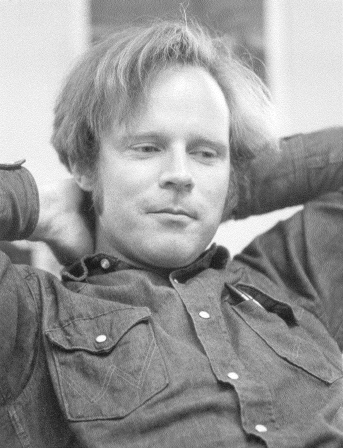
\includegraphics[width=1.5in]{Floyd.png}
%		\caption{R. W. Floyd [1964]}
%	\end{figure}
%		
%}

\frame{
	\frametitle{Tree implementation: {\sc Find} }
	\begin{itemize}
	           \item Basic idea: We use a tree to store elements of a set, and use root as ``set name". Thus, only one representative should be maintained. 

\begin{figure}
\begin{tikzpicture}[scale=1., auto,swap]

  \def\dx{0};
  \def\dy{0}; 
 \def\u{0.8};
  
   \foreach \x/\y/\name/\label in { 0/0/root/s, 0/-1/L11/a, 1/-1/L12/b, 1/-2/L21/c}
          \node[smallvertex,draw=black, fill=blue!20] (\name) at (\x*\u+\dx, \y + \dy) {\tiny $\label$};
  
  \foreach \source/ \dest /\weight in {L11/root/{}, L12/root/{}}
         \draw[->] (\source) -- node[weight] {$\weight$} (\dest);

  \foreach \source/ \dest /\weight in {L21/L12/{}}
         \draw[->] (\source) -- node[weight] {$\weight$} (\dest);

   \foreach \x/\y/\name/\label in { 0/0/root/s }
          \node[smallvertex,draw=black, fill=blue!20] (\name) at (\x*\u+\dx, \y + \dy) {\tiny $\label$} edge [out=135, in=45, loop] ();

  \node[blue, ultra thick] at (-2, 0) {Set: $\{s, a, b, c \}$};
    
   \end{tikzpicture}
\end{figure}
\item Operation: 
	
	{\sc Find}$(x)$
\begin{algorithmic}[1]
\STATE $r = x$; 
\WHILE { $r != parent(r) $}
\STATE $r = parent(r)$; 
\ENDWHILE
\RETURN $r$; 
\end{algorithmic}
%\item Complexity: O(n)
\end{itemize}
}


\frame{
	\frametitle{Tree implementation: {\sc Union} }

\begin{itemize}

\item Operation: 

	{\sc Union}$(x, y)$
\begin{algorithmic}[1]
\STATE $r_x = ${\sc Find}$(x)$; 
\STATE $r_y = ${\sc Find}$(y)$;
\STATE $parent(r_x) = r_y$; 
\end{algorithmic}
%\item Complexity: O(n)
\item Example: {\sc Union}$(c, a)$
\end{itemize}


\begin{figure}
\begin{tikzpicture}[scale=1., auto,swap]


  \def\dx{0};
  \def\dy{0}; 
 \def\u{0.8};
  
   \foreach \x/\y/\name/\label in { -5/0/root/s, -5/-1/L11/a, -3.5/0/L12/b, -3.5/-1/L21/c}
          \node[smallvertex,draw=black, fill=blue!20] (\name) at (\x*\u+\dx, \y + \dy) {\tiny $\label$};
  
  \foreach \source/ \dest /\weight in {L11/root/{}}
         \draw[->] (\source) -- node[weight] {$\weight$} (\dest);

  \foreach \source/ \dest /\weight in {L21/L12/{}}
         \draw[->] (\source) -- node[weight] {$\weight$} (\dest);

   \foreach \x/\y/\name/\label in { -5/0/root/s }
          \node[smallvertex,draw=black, fill=blue!20] (\name) at (\x*\u+\dx, \y + \dy) {\tiny $\label$} edge [out=135, in=45, loop] ();

   \foreach \x/\y/\name/\label in { -3.5/0/root/b }
          \node[smallvertex,draw=black, fill=blue!20] (\name) at (\x*\u+\dx, \y + \dy) {\tiny $\label$} edge [out=135, in=45, loop] ();


   \draw[->, line width=2pt, blue] (-2.5, -0.5) -- node[above]{{\sc Union}$(c, a)$} (-0.5, -0.5); 

  \def\dx{0};
  \def\dy{0}; 
 \def\u{0.8};
  
   \foreach \x/\y/\name/\label in { 0/0/root/s, 0/-1/L11/a, 1/-1/L12/b, 1/-2/L21/c}
          \node[smallvertex,draw=black, fill=blue!20] (\name) at (\x*\u+\dx, \y + \dy) {\tiny $\label$};
  
  \foreach \source/ \dest /\weight in {L11/root/{}, L12/root/{}}
         \draw[->] (\source) -- node[weight] {$\weight$} (\dest);

  \foreach \source/ \dest /\weight in {L21/L12/{}}
         \draw[->] (\source) -- node[weight] {$\weight$} (\dest);

   \foreach \x/\y/\name/\label in { 0/0/root/s }
          \node[smallvertex,draw=black, fill=blue!20] (\name) at (\x*\u+\dx, \y + \dy) {\tiny $\label$} edge [out=135, in=45, loop] ();

%  \node[blue, ultra thick] at (3, 0) {Set: $\{s, a, b, c \}$};
    
   \end{tikzpicture}
\end{figure}
}


\frame{
	\frametitle{Tree implementation: worst case}
%	\begin{itemize}
%	           \item Basic idea: using a tree to store elements of a set, and using root as set name. 


 


\begin{itemize}
	\item Worst case: the tree degenerates into a linked list. For example, {\sc Union}$(c, b)$, {\sc Union}$(b, a)$, {\sc Union}$(a, s)$. 

\begin{figure}
\begin{tikzpicture}[scale=1., auto,swap]

  \def\dx{0};
  \def\dy{0}; 
  \def\u{0.8};
  


   \foreach \x/\y/\name/\label in { -5/-1.5/root/c }
          \node[smallvertex,draw=black, fill=blue!20] (\name) at (\x*\u+\dx, \y + \dy) {\tiny $\label$} edge [out=135, in=45, loop] ();

   \foreach \x/\y/\name/\label in { -6/-1.5/root/b }
          \node[smallvertex,draw=black, fill=blue!20] (\name) at (\x*\u+\dx, \y + \dy) {\tiny $\label$} edge [out=135, in=45, loop] ();

   \foreach \x/\y/\name/\label in { -7/-1.5/root/a }
          \node[smallvertex,draw=black, fill=blue!20] (\name) at (\x*\u+\dx, \y + \dy) {\tiny $\label$} edge [out=135, in=45, loop] ();

   \foreach \x/\y/\name/\label in { -8/-1.5/root/s }
          \node[smallvertex,draw=black, fill=blue!20] (\name) at (\x*\u+\dx, \y + \dy) {\tiny $\label$} edge [out=135, in=45, loop] ();


   \draw[->, line width=2pt, blue] (-3, -1.5) -- (-0.5, -1.5);
   \node[blue, ultra thick] at (-1.75, 0) { {\sc Union}$( c, b)$ };
   \node[blue, ultra thick] at (-1.75, -0.5) { {\sc Union}$( b, a)$ };
     \node[blue, ultra thick] at (-1.75, -1) { {\sc Union}$( a, s)$ };
    
%   \draw[->, line width=2pt, blue] (-3, -0.5) -- node[above]{{\sc Union}$( c, b)$ \\ {\sc Union}$( b, a)$ {\sc Union}$(a, s)$ } (-0.5, -0.5); 


   \foreach \x/\y/\name/\label in { 0/0/root/s, 0/-1/L11/a, 0/-2/L12/b, 0/-3/L13/c}
          \node[smallvertex,draw=black, fill=blue!20] (\name) at (\x*\u+\dx, \y + \dy) {\tiny $\label$};
  
  \foreach \source/ \dest /\weight in {L11/root/{}, L12/L11/{}, L13/L12/{}}
         \draw[->] (\source) -- node[weight] {$\weight$} (\dest);

   \foreach \x/\y/\name/\label in { 0/0/root/s }
          \node[smallvertex,draw=black, fill=blue!20] (\name) at (\x*\u+\dx, \y + \dy) {\tiny $\label$} edge [out=135, in=45, loop] ();

%  \node[blue, ultra thick] at (-2, 0) {Set: $\{s, a, b, c \}$};
    
   \end{tikzpicture}
   
\end{figure}

		\item Complexity: {\sc Find} takes $O(n)$ time, 	and  {\sc Union} takes  $O(n)$ time. 
 		\item Question: how to keep a ``good" tree shape to limit path length? 
\end{itemize}
}


\frame{
	\begin{block}{}
	Link-by-rank: shorten the path by maintaining a balanced tree
	%	 root to represent set name
	%  (J. W. J. Williams, 1964, R. W. Floyd, 1964)
	\end{block}
} 

\frame{
	\frametitle{Tree implementation with link-by-size}
	\begin{itemize}
	           \item Basic idea: We shorten the path by maintaining a balanced-tree. In fact, this will limit path length to $O(\log n)$. 
	           \item How to maintain a balanced tree? Each node is associated with a $rank$, denoting its height. The tree has a balanced shape via linking smaller tree to larger tree; if tie, increase the rank of new root by $1$. 
	\end{itemize}
	

\begin{figure}
\begin{tikzpicture}[scale=1., auto,swap]


  \def\dx{0};
  \def\dy{0}; 
 \def\u{0.8};
  
   \foreach \x/\y/\name/\label in { -4.5/0/root/s^0, -3/0/a/a^0, -1.5/0/b/b^1, -1.5/-1/c/c^0}
          \node[middlevertex,draw=black, fill=blue!20] (\name) at (\x*\u+\dx, \y + \dy) {\tiny $\label$};
  
  \foreach \source/ \dest /\weight in {c/b/{}}
         \draw[->] (\source) -- node[weight] {$\weight$} (\dest);

   \foreach \x/\y/\name/\label in { -4.5/0/root/s^0}
          \node[middlevertex,draw=black, fill=blue!20] (\name) at (\x*\u+\dx, \y + \dy) {\tiny $\label$} edge [out=135, in=45, loop] ();

   \foreach \x/\y/\name/\label in { -3/0/root/a^0}
          \node[middlevertex,draw=black, fill=blue!20] (\name) at (\x*\u+\dx, \y + \dy) {\tiny $\label$} edge [out=135, in=45, loop] ();


   \foreach \x/\y/\name/\label in { -1.5/0/root/b^1}
          \node[middlevertex,draw=black, fill=blue!20] (\name) at (\x*\u+\dx, \y + \dy) {\tiny $\label$} edge [out=135, in=45, loop] ();

%  \node[blue, ultra thick] at (-2, 0) {Set: $\{s, a, b, c \}$};

   
   \end{tikzpicture}
   \caption{Three sets: \{$s$\}, \{$a$\},  \{$b, c$\} }
\end{figure}
	
} 


\frame{
	\frametitle{Tree implementation with link-by-size: {\sc Union} operation}

\begin{small}
	{\sc Union}$(x, y)$
\begin{algorithmic}[1]
\STATE $r_x = ${\sc Find}$(x)$; 
\STATE $r_y = ${\sc Find}$(y)$;
\IF{ $rank(r_x) > rank(r_y)$}
\STATE $parent(r_y) = r_x$;
\ELSE
	\STATE $parent(r_x) = r_y$;
	\IF{ $rank(r_x) == rank(r_y)$}
			\STATE $rank(r_y) = rank(r_y)+1$;
	\ENDIF
\ENDIF
\end{algorithmic}
\end{small}


\begin{figure}
\begin{tikzpicture}[scale=1., auto,swap]

  \def\dx{0};
  \def\dy{0}; 
  \def\u{0.8};
  


   \foreach \x/\y/\name/\label in { -5/-1.5/root/c^0 }
          \node[middlevertex,draw=black, fill=blue!20] (\name) at (\x*\u+\dx, \y + \dy) {\tiny $\label$} edge [out=135, in=45, loop] ();

   \foreach \x/\y/\name/\label in { -6.5/-1.5/root/b^0 }
          \node[middlevertex,draw=black, fill=blue!20] (\name) at (\x*\u+\dx, \y + \dy) {\tiny $\label$} edge [out=135, in=45, loop] ();

   \foreach \x/\y/\name/\label in { -8/-1.5/root/a^0 }
          \node[middlevertex,draw=black, fill=blue!20] (\name) at (\x*\u+\dx, \y + \dy) {\tiny $\label$} edge [out=135, in=45, loop] ();

   \foreach \x/\y/\name/\label in { -9.5/-1.5/root/s^0 }
          \node[middlevertex,draw=black, fill=blue!20] (\name) at (\x*\u+\dx, \y + \dy) {\tiny $\label$} edge [out=135, in=45, loop] ();


   \draw[->, line width=2pt, blue] (-3, -1.5) -- (-0.5, -1.5);
   \node[blue, ultra thick] at (-1.75, 0) { {\sc Union}$( c, b)$ };
   \node[blue, ultra thick] at (-1.75, -0.5) { {\sc Union}$( b, a)$ };
     \node[blue, ultra thick] at (-1.75, -1) { {\sc Union}$( a, s)$ };
    
%   \draw[->, line width=2pt, blue] (-3, -0.5) -- node[above]{{\sc Union}$( c, b)$ \\ {\sc Union}$( b, a)$ {\sc Union}$(a, s)$ } (-0.5, -0.5); 


   \foreach \x/\y/\name/\label in { 0/-1/root/b^1, 0/-2/c/c^0, 1/-2/a/a^0, 2/-2/s/s^0}
          \node[middlevertex,draw=black, fill=blue!20] (\name) at (\x*\u+\dx, \y + \dy) {\tiny $\label$};
  
  \foreach \source/ \dest /\weight in {c/root/{}, a/root/{}, s/root/{}}
         \draw[->] (\source) -- node[weight] {$\weight$} (\dest);

   \foreach \x/\y/\name/\label in { 0/-1/root/b^1 }
          \node[middlevertex,draw=black, fill=blue!20] (\name) at (\x*\u+\dx, \y + \dy) {\tiny $\label$} edge [out=135, in=45, loop] ();

%  \node[blue, ultra thick] at (-2, 0) {Set: $\{s, a, b, c \}$};
    
   \end{tikzpicture}
   
\end{figure}
Note: a node's rank will not change after it becomes an internal node. 
}


\frame[allowframebreaks]{
	\frametitle{ Properties of rank }
\begin{enumerate}
\item For any node $x$, $rank(x) < rank( parent(x))$.
\item Any tree with root rank of $k$ contains at least $2^k$ nodes. (Hint: by induction on $k$.) 
\item Once a root node was changed into internal node during a {\sc Union} operation, its  rank will not change afterwards. 
\begin{figure}
\begin{tikzpicture}[scale=1., auto,swap]



  \def\dx{0};
  \def\dy{0}; 
  
   \draw[thick, fill=green!20] (0, 0) -- (-0.5, -0.73) -- (0.5, -0.73) -- (0,0); 
  % \node[ thick, blue] at (0, -0.48-0.5) {rank: $k$};
   \draw[thick, fill=green!20] (1.5+0, 0-1) -- (1.5-0.5, -0.73-1) -- (1.5+0.5, -0.73-1) -- (1.5+0,0-1); 
   \node[ thick, blue] at (0+2.5, -0.48-0.5) {rank: $k$};

  
   \foreach \x/\y/\name/\label in { 0/0/root/, 1.5/-1/L11/}
          \node[tinyvertex,draw=black, fill=white!20] (\name) at (\x+\dx, \y + \dy) {\tiny $\label$};
  
   \node[ thick, blue, above ] at (root.north) { rank: ${k+1}$};
  

  
  \foreach \source/ \dest /\weight in {root/L11/{}}
         \path[undirectededge] (\source) -- node[weight] {$\weight$} (\dest);
 


   \foreach \x/\y/\name/\label in { -2/0/root/}
          \node[tinyvertex,draw=black, fill=white!20] (\name) at (\x+\dx, \y + \dy) {\tiny $\label$};

  
   \node[ thick, blue, above ] at (root.north) { rank: ${0}$};
  

   \end{tikzpicture}
\end{figure}

\item Suppose we have $n$ elements. The number of rank $k$ nodes is at most $\frac{n}{2^k}$. (Hint: Different nodes of rank $k$ share no common descendants.)
\end{enumerate}

\begin{figure}
\begin{tikzpicture}[scale=1., auto,swap]

  \def\dx{0};
  \def\dy{0}; 
  \def\u{0.8};
  
     \foreach \x/\y/\name/\label in {  -1/-1/R11/b^{1}, -1/-2/R21/i^{0}, -2/-2/R22/h^{0}, -3/-2/R23/g^{0}} 
          \node[middlevertex,draw=black, fill=white!20] (\name) at (\x*\u+\dx, \y + \dy) {\tiny $\label$};

  
   \foreach \x/\y/\name/\label in { 0/0/root/a^{4}, 0/-1/L11/c^{0}, 1/-1/L12/d^{1}, 2/-1/L13/e^{2}, 4/-1/L14/f^{3}} 
          \node[middlevertex,draw=black, fill=white!20] (\name) at (\x*\u+\dx, \y + \dy) {\tiny $\label$};
  
   \foreach \x/\y/\name/\label in {1/-2/L21/j^{0}, 2/-2/L22/k^{0}, 3/-2/L23/l^{1}, 4/-2/L24/m^{0}, 5/-2/L25/n^{1}, 6/-2/L26/o^{2}}
          \node[middlevertex,draw=black, fill=white!20] (\name) at (\x*\u+\dx, \y + \dy) {\tiny $\label$};

   \foreach \x/\y/\name/\label in {3/-3/L31/p^{0}, 5/-3/L32/q^{0}, 6/-3/L33/r^{0}, 7/-3/L34/s^{1}}
          \node[middlevertex,draw=black, fill=white!20] (\name) at (\x*\u+\dx, \y + \dy) {\tiny $\label$};


   \foreach \x/\y/\name/\label in {7/-4/L41/t^{0}}
          \node[middlevertex,draw=black, fill=white!20] (\name) at (\x*\u+\dx, \y + \dy) {\tiny $\label$};

   \foreach \x/\y/\name/\label in { 0/0/root/a^{4} }
          \node[middlevertex,draw=black, fill=red!20] (\name) at (\x*\u+\dx, \y + \dy) {\tiny $\label$} edge [out=135, in=45, loop] ();
       
              \foreach \x/\y/\name/\label in {4/-1/L14/f^{3} }
          \node[middlevertex,draw=black, fill=yellow!20] (\name) at (\x*\u+\dx, \y + \dy) {\tiny $\label$};  
         
              \foreach \x/\y/\name/\label in {6/-2/L26/o^{2}, 2/-1/L13/e^{2} }
          \node[middlevertex,draw=black, fill=blue!20] (\name) at (\x*\u+\dx, \y + \dy) {\tiny $\label$};  
         
         
       \foreach \x/\y/\name/\label in { 7/-3/L34/s^{1}, -1/-1/R11/b^{1}, 1/-1/L12/d^{1}, 3/-2/L23/l^{1}, 5/-2/L25/n^{1}}
          \node[middlevertex,draw=black, fill=green!20] (\name) at (\x*\u+\dx, \y + \dy) {\tiny $\label$};
      
          
  
  \foreach \source/ \dest /\weight in {root/L11/{}, root/L12/{}, root/L13/{}, root/L14/{}}
         \path[undirectededge] (\source) -- node[weight] {$\weight$} (\dest);
         
     \foreach \source/ \dest /\weight in {root/R11/{}, R11/R21/{}, R11/R22/{}, R11/R23/{}}
         \path[undirectededge] (\source) -- node[weight] {$\weight$} (\dest);      
 
  \foreach \source/ \dest /\weight in {L12/L21/{}, L13/L22/{}, L13/L23/{}, L14/L24/{}, L14/L25/{}, L14/L26/{}, L23/L31/{}, L25/L32/{}, L26/L33/{}, L26/L34/{}, L34/L41/{}}
         \path[undirectededge] (\source) -- node[weight] {$\weight$} (\dest);
 

 \node[ blue, thick] at (2, 0) { {\small rank 4: 1 nodes} };
 \node[ blue, thick] at (5, -1) {{\small rank 3: 1 nodes }};
 \node[ blue, thick] at (6.5, -2) {{\small rank 2:  2 nodes }};
 \node[ blue, thick] at (7.2, -3) {{\small rank 1: 5 nodes }};
   \node[ blue, thick] at (7.2, -4) {{\small rank 0: 11 nodes }};
    
   \end{tikzpicture}
\end{figure}

\begin{itemize}
\item 
Thus, all of the trees have height less than $\log n$, which means both  {\sc Find} and {\sc Union} take  $O(\log n)$ time. 
\end{itemize}

}



\frame{
	\begin{block}{}
	Path compression: compress paths to make further {\sc Find} efficient
%	 root to represent set name
	%  (J. W. J. Williams, 1964, R. W. Floyd, 1964)
	\end{block}
} 

\frame{
	\frametitle{Path compression} 

\begin{itemize}
	\item Basic idea: After finding the root $r$ of the tree containing $x$, we change the parent of the nodes along the path to point directly to $r$.  Thus, the subsequent {\sc Find}$(x)$ operations will be efficient. 



\begin{figure}
\begin{tikzpicture}[scale=0.9, auto,swap]



  \def\dx{0};
  \def\dy{0}; 
  
   \draw[thick, fill=green!20] (0, 0) -- (-0.5, -0.73) -- (0.5, -0.73) -- (0,0); 
   \node[ thick, blue] at (0, -0.48) { $T_{1}$};
  
   \draw[thick, fill=green!20] (1.5+0, 0-1) -- (1.5-0.5, -0.73-1) -- (1.5+0.5, -0.73-1) -- (1.5+0,0-1); 
   \node[ thick, blue] at (0+1.5, -0.48-1) {$T_{2}$};

     \draw[thick, fill=green!20] (1.5+1.5+0, 0-1-1) -- (1.5+1.5-0.5, -0.73-1-1) -- (1.5+1.5+0.5, -0.73-1-1) -- (1.5+1.5+0,0-1-1); 
   \node[ thick, blue] at (0+1.5+1.5, -0.48-1-1) {$T_{3}$};

  
  
   \foreach \x/\y/\name/\label in { 0/0/root/r, 1.5/-1/L11/x, 1.5+1.5/-1-1/L12/y}
          \node[smallvertex,draw=black, fill=white!20] (\name) at (\x+\dx, \y + \dy) {\tiny $\label$};
  
%   \node[ thick, blue, above ] at (root.north) { $B_{k+1}$};
  

  \foreach \source/ \dest /\weight in {root/L11/{}, L11/L12/{}}
         \path[undirectededge] (\source) -- node[weight] {$\weight$} (\dest);
 
%   \foreach \x/\y/\name/\label in { -2/0/root/}
%          \node[tinyvertex,draw=black, fill=white!20] (\name) at (\x+\dx, \y + \dy) {\tiny $\label$};
% \node[ thick, blue, above ] at (root.north) { $B_{0}$};
  
\draw[->, line width=2pt, blue] (3, -1) -- node[above]{{\sc Find}$(y)$} (4.5, -1); 

     \foreach \x/\y/\name/\label in { 0/0/root/r }
          \node[smallvertex,draw=black, fill=blue!20] (\name) at (\x+\dx, \y + \dy) {\tiny $\label$} edge [out=135, in=45, loop] ();
          
  \def\dx{5.5};
  \def\dy{0}; 
  
   \draw[thick, fill=green!20] (0+\dx, 0) -- (-0.5+\dx, -0.73) -- (0.5+\dx, -0.73) -- (0+\dx,0); 
   \node[ thick, blue] at (0+\dx, -0.48) { $T_{1}$};
  
   \draw[thick, fill=green!20] (1.5+0+\dx, 0-1) -- (1.5-0.5+\dx, -0.73-1) -- (1.5+0.5+\dx, -0.73-1) -- (1.5+0+\dx,0-1); 
   \node[ thick, blue] at (0+1.5+\dx, -0.48-1) {$T_{2}$};

     \draw[thick, fill=green!20] (1.5+1.5+0+\dx, 0-1) -- (1.5+1.5-0.5+\dx, -0.73-1) -- (1.5+1.5+0.5+\dx, -0.73-1) -- (1.5+1.5+0+\dx,0-1); 
   \node[ thick, blue] at (0+1.5+1.5+\dx, -0.48-1) {$T_{3}$};

  
     \foreach \x/\y/\name/\label in { 0/0/root/r }
          \node[smallvertex,draw=black, fill=white!20] (\name) at (\x+\dx, \y + \dy) {\tiny $\label$} edge [out=135, in=45, loop] ();

  
   \foreach \x/\y/\name/\label in { 0/0/root/r, 1.5/-1/L11/x, 1.5+1.5/-1/L12/y}
          \node[smallvertex,draw=black, fill=white!20] (\name) at (\x+\dx, \y + \dy) {\tiny $\label$};
  
%   \node[ thick, blue, above ] at (root.north) { $B_{k+1}$};
  

  \foreach \source/ \dest /\weight in {root/L11/{}, root/L12/{}}
         \path[undirectededge] (\source) -- node[weight] {$\weight$} (\dest);
 
%   \foreach \x/\y/\name/\label in { -2/0/root/}
%          \node[tinyvertex,draw=black, fill=white!20] (\name) at (\x+\dx, \y + \dy) {\tiny $\label$};
% \node[ thick, blue, above ] at (root.north) { $B_{0}$};
  
   \end{tikzpicture}
\end{figure}
	\item Note: Path compression changes height of nodes but does not change rank of nodes. We always have $height(x) \leq rank(x)$; thus, the three properties still hold.  
\end{itemize}

 

}

\frame{
	\frametitle{Path compression: {\sc Find} operation } 



\begin{figure}
\begin{tikzpicture}[scale=0.9, auto,swap]



  \def\dx{0};
  \def\dy{0}; 
  
   \draw[thick, fill=green!20] (0, 0) -- (-0.5, -0.73) -- (0.5, -0.73) -- (0,0); 
   \node[ thick, blue] at (0, -0.48) { $T_{1}$};
  
   \draw[thick, fill=green!20] (1.5+0, 0-1) -- (1.5-0.5, -0.73-1) -- (1.5+0.5, -0.73-1) -- (1.5+0,0-1); 
   \node[ thick, blue] at (0+1.5, -0.48-1) {$T_{2}$};

     \draw[thick, fill=green!20] (1.5+1.5+0, 0-1-1) -- (1.5+1.5-0.5, -0.73-1-1) -- (1.5+1.5+0.5, -0.73-1-1) -- (1.5+1.5+0,0-1-1); 
   \node[ thick, blue] at (0+1.5+1.5, -0.48-1-1) {$T_{3}$};

  
  
   \foreach \x/\y/\name/\label in { 0/0/root/r, 1.5/-1/L11/x, 1.5+1.5/-1-1/L12/y}
          \node[smallvertex,draw=black, fill=white!20] (\name) at (\x+\dx, \y + \dy) {\tiny $\label$};
  
%   \node[ thick, blue, above ] at (root.north) { $B_{k+1}$};
  

  \foreach \source/ \dest /\weight in {root/L11/{}, L11/L12/{}}
         \path[undirectededge] (\source) -- node[weight] {$\weight$} (\dest);
 
%   \foreach \x/\y/\name/\label in { -2/0/root/}
%          \node[tinyvertex,draw=black, fill=white!20] (\name) at (\x+\dx, \y + \dy) {\tiny $\label$};
% \node[ thick, blue, above ] at (root.north) { $B_{0}$};
  
\draw[->, line width=2pt, blue] (3, -1) -- node[above]{{\sc Find}$(y)$} (4.5, -1); 

     \foreach \x/\y/\name/\label in { 0/0/root/r }
          \node[smallvertex,draw=black, fill=blue!20] (\name) at (\x+\dx, \y + \dy) {\tiny $\label$} edge [out=135, in=45, loop] ();
          
  \def\dx{5.5};
  \def\dy{0}; 
  
   \draw[thick, fill=green!20] (0+\dx, 0) -- (-0.5+\dx, -0.73) -- (0.5+\dx, -0.73) -- (0+\dx,0); 
   \node[ thick, blue] at (0+\dx, -0.48) { $T_{1}$};
  
   \draw[thick, fill=green!20] (1.5+0+\dx, 0-1) -- (1.5-0.5+\dx, -0.73-1) -- (1.5+0.5+\dx, -0.73-1) -- (1.5+0+\dx,0-1); 
   \node[ thick, blue] at (0+1.5+\dx, -0.48-1) {$T_{2}$};

     \draw[thick, fill=green!20] (1.5+1.5+0+\dx, 0-1) -- (1.5+1.5-0.5+\dx, -0.73-1) -- (1.5+1.5+0.5+\dx, -0.73-1) -- (1.5+1.5+0+\dx,0-1); 
   \node[ thick, blue] at (0+1.5+1.5+\dx, -0.48-1) {$T_{3}$};

  
     \foreach \x/\y/\name/\label in { 0/0/root/r }
          \node[smallvertex,draw=black, fill=white!20] (\name) at (\x+\dx, \y + \dy) {\tiny $\label$} edge [out=135, in=45, loop] ();

  
   \foreach \x/\y/\name/\label in { 0/0/root/r, 1.5/-1/L11/x, 1.5+1.5/-1/L12/y}
          \node[smallvertex,draw=black, fill=white!20] (\name) at (\x+\dx, \y + \dy) {\tiny $\label$};
  
%   \node[ thick, blue, above ] at (root.north) { $B_{k+1}$};
  

  \foreach \source/ \dest /\weight in {root/L11/{}, root/L12/{}}
         \path[undirectededge] (\source) -- node[weight] {$\weight$} (\dest);
 
%   \foreach \x/\y/\name/\label in { -2/0/root/}
%          \node[tinyvertex,draw=black, fill=white!20] (\name) at (\x+\dx, \y + \dy) {\tiny $\label$};
% \node[ thick, blue, above ] at (root.north) { $B_{0}$};
  
   \end{tikzpicture}
\end{figure}

 
	{\sc Find}$(x)$
\begin{algorithmic}[1]
\IF{$x  != parent(x) $}
\STATE $parent(x) = $ {\sc Find}$(parent(x) )$; 
\ELSE
\RETURN {$x$}; 
\ENDIF 
\end{algorithmic}


}

\frame{
	\frametitle{Some properties of {\sc Find} and {\sc Union}}
	
	\begin{itemize}
		\item {\sc Find} operations change internal nodes only while {\sc Union} operations change root node only. 
		\item Path compression changes parent node of certain internal nodes. However, it will not change the root nodes, rank of any node, and thus will not  affect {\sc Union} operations. 
	\end{itemize}
}

\frame{
	\frametitle{Path compression: complexity} 



\begin{itemize}
	\item Example: {\sc Find}$(c)$
\end{itemize}

\begin{figure}
\begin{tikzpicture}[scale=1., auto,swap]


  \def\dx{-1};
  \def\dy{0}; 
 \def\u{0.8};
  
   \foreach \x/\y/\name/\label in { 0/0/root/s^2, 0/-1/L11/a^0, 1/-1/L12/b^1, 1/-2/L21/c^0}
          \node[middlevertex,draw=black, fill=blue!20] (\name) at (\x*\u+\dx, \y + \dy) {\tiny $\label$};
  
  \foreach \source/ \dest /\weight in {L11/root/{}, L12/root/{}}
         \draw[->] (\source) -- node[weight] {$\weight$} (\dest);

  \foreach \source/ \dest /\weight in {L21/L12/{}}
         \draw[->] (\source) -- node[weight] {$\weight$} (\dest);

   \foreach \x/\y/\name/\label in { 0/0/root/s^{2} }
          \node[middlevertex,draw=black, fill=blue!20] (\name) at (\x*\u+\dx, \y + \dy) {\tiny $\label$} edge [out=135, in=45, loop] ();


   \draw[->, line width=2pt, blue] (0.5, -0.5) -- node[above]{{\sc Find}$(c)$} (2.5, -0.5); 

  \def\dx{3};
  \def\dy{0}; 
 \def\u{0.8};
  
   \foreach \x/\y/\name/\label in { 0/0/root/s^2, 0/-1/L11/a^0, 1/-1/L12/b^1, 2/-1/L21/c^0}
          \node[middlevertex,draw=black, fill=blue!20] (\name) at (\x*\u+\dx, \y + \dy) {\tiny $\label$};
  
  \foreach \source/ \dest /\weight in {L11/root/{}, L12/root/{}}
         \draw[->] (\source) -- node[weight] {$\weight$} (\dest);

  \foreach \source/ \dest /\weight in {L21/root/{}}
         \draw[->] (\source) -- node[weight] {$\weight$} (\dest);

   \foreach \x/\y/\name/\label in { 0/0/root/s^{2} }
          \node[middlevertex,draw=black, fill=blue!20] (\name) at (\x*\u+\dx, \y + \dy) {\tiny $\label$} edge [out=135, in=45, loop] ();

    
   \end{tikzpicture}
\end{figure}

	\begin{itemize}
		\item A {\sc Find}$(c)$ operation might takes long time; however, the path compression makes subsequent {\sc Find}$(c)$ (and other middle nodes in the path) efficient.   
%		\item After path compression, ``rank" is not exactly the height of sub-tree; however, the three properties still hold.  
\end{itemize}

\begin{theorem}
	Starting from each item forming an individual set, any sequence of $m$ operations (including {\sc Find} and {\sc Union}) over $n$ elements takes   $O(m \log^* n)$ time. 
\end{theorem}
}


\frame{
	\frametitle{Analysis of path compression: a brief history } 
	
	\begin{itemize}
		\item In 1972, Fischer proved a bound of $O( m \log \log n)$. 
		\item In 1973, Hopcroft and Ullman proved a bound of $O(m\log^{*} n)$. 
		\item In 1975, R. Tarjan et al. proved a bound using ``inverse Ackerman function''. 
		\item Later, R. Tarjan, et. al. and Harfst and Reingold proved the bound using the potential function technique. 
	\end{itemize}
	Here, we present the proof in {\it Algorithms}  by S. Dasgupta, C.
H. Papadimitriou, and U. V. Vazirani. 
} 

\frame{
	\frametitle{$\log^*n$: Iterated logarithm function} 
\begin{itemize}
	\item Intuition: the number of logarithm operations to make $n$ to be $1$. 
	\item  
	$\log^*n = \begin{cases} 0 & \text{if } n = 1 \\ 
	                                    1+\log^*(\log n ) & \text{otherwise} 
	                                    \end{cases} $

\begin{table}
{ \begin{tabular}{cc}\hline
       $n$ & $\log^* n$\\
 \hline
 1 & 0 \\ 
2 & 1 \\ 
$ [3, 2^2]$ & 2 \\ 
 $[5, 2^4]$ & 3 \\ 
$ [17, 2^{16}]$ & 4 \\ 
 $[65537, 2^{65536}]$ & 5 \\ 
\hline
     \end{tabular}} {}%
 \end{table}

 	\item Note: $\log^*n$ increases very slowly, and we have $\log^*n < 5$ unless $n$ exceeds the number of atoms in the universe. 
 \end{itemize}

} 

\frame{
	\frametitle{Analysis of rank} 

	\begin{itemize}
		\item Let's divide the nonzero ranks into groups as below. 

\begin{table}
{ \begin{tabular}{ccc}\hline
  Group     & Rank  & Upper bound of $\#$elements \\
 \hline
0&  1 & $   \frac{n}{2}$ \\ 
1& 2 & $  \frac{n}{2^{2}}$ \\ 
2& $[3, 2^2]$ & $   \frac{n}{2^{2}}$  \\ 
3& $[5, 2^4]$ & $  \frac{n}{2^{4}}$  \\ 
4 & $[17, 2^{16}]$ & $   \frac{n}{2^{16}}$ \\ 
 5& $[65537, 2^{65536}]$ & $  \frac{n}{2^{65536}}$ \\ 
\hline
     \end{tabular}} {}%
 \end{table}
 
 	\item Note: 
 		\begin{itemize}
			\item Group number is $\log^* rank$ and  the number of groups is at most $\log^{*} n$.
			\item The  number of elements in the rank group $G_k$ ($k\geq 2$) is  at most $\frac{n}{ \underbrace{
  {{{{2\vphantom{h}}}^{2\vphantom{h}}}^{\cdots\vphantom{h}}}^{2\vphantom{h}}
}_{\text{k}} }$ as the number of nodes with rank $r$ is at most $\frac{n}{2^{r}}$. We will see why the group was set to take the form $[ \underbrace{
  {{{{2\vphantom{h}}}^{2\vphantom{h}}}^{\cdots\vphantom{h}}}^{2\vphantom{h}}
}_{\text{k-1}} + 1  ,  \underbrace{
  {{{{2\vphantom{h}}}^{2\vphantom{h}}}^{\cdots\vphantom{h}}}^{2\vphantom{h}}
}_{\text{k}}]$ soon.  

		\end{itemize}
\end{itemize}
} 

\frame{
	\frametitle{Amortized analysis: total time of $m$ {\sc Find} operations} 

\begin{itemize}
	\item Basic idea: a {\sc Find} operation might take long time; however, path compression makes subsequent {\sc Find} operations efficient. 
	\item Let's consider a sequence of $m$ {\sc Find} operations, and divide the traversed links into the following three types:   
		\begin{itemize}
			\item \textcolor{green}{\bf Type 1:} links to \textcolor{green}{\bf root}
			\item \textcolor{red}{\bf Type 2:} links traversed \textcolor{red}{\bf between} different rank groups
			\item \textcolor{blue}{\bf Type 3:} links traversed \textcolor{blue}{\bf within} the same rank groups
		\end{itemize}
	\item For example, the links that {\sc Find}$(a)$ travels: 
\begin{figure}
\begin{tikzpicture}[scale=1., auto,swap]

  \def\dx{0};
  \def\dy{0}; 
  \def\u{1};
  
     \foreach \y/\x/\name/\label in {  0/1/b/b^{1}, 0/2/c/c^{2}, 0/3/d/d^{3}, 0/4/e/e^{4}, 0/5/f/f^{5}, 0/6/g/g^{6},  0/7/h/h^{7}, 0/8/i/i^{8}} 
     	\draw[thick, fill=green!20] (\x+\dx, \y+\dy) -- (\x-0.4+\dx, \y-0.73+\dy) -- (\x+0.4+\dx, \y-0.73+\dy) -- (\x+\dx, \y+\dy);
     \foreach \y/\x/\name/\label in {  0/1/b/T_{1}, 0/2/c/T_{2}, 0/3/d/T_{3}, 0/4/e/T_{4}, 0/5/f/T_{5}, 0/6/g/T_{6},  0/7/h/T_{7}, 0/8/i/T_{8}} 
     	 \node[ thick, blue] at (\x+\dx, \y-0.5+\dy) {\tiny $\label$};

   \foreach \y/\x/\name/\label in { 0/0/a/a^{0}, 0/1/b/b^{1}, 0/2/c/c^{2}, 0/3/d/d^{3}, 0/4/e/e^{4}, 0/5/f/f^{5}, 0/6/g/g^{6},  0/7/h/h^{7}, 0/8/i/i^{8}} 
          \node[smallvertex,draw=black, fill=white!20] (\name) at (\x*\u+\dx, \y + \dy) {\tiny $\label$};
  
%	
%    \foreach \y/\x/\name/\label in {  0/7/h/h^7,0/8/i/i^8} 
%          \node[smallvertex,draw=black, fill=white!20] (\name) at (\x*\u+\dx, \y + \dy) {\tiny $\label$};
 
  \foreach \source/ \dest /\weight in {a/b/{}, b/c/{}, c/d/{}, e/f/{}}
         \draw[->, thick, red] (\source) -- node[weight] {$\weight$} (\dest);
    \foreach \source/ \dest /\weight in {d/e/{}, f/g/{}, g/h/{}}
         \draw[->, thick, blue] (\source) -- node[weight] {$\weight$} (\dest);
    \foreach \source/ \dest /\weight in {h/i/{}}
         \draw[->, thick, green] (\source) -- node[weight] {$\weight$} (\dest);
        
%          \node[black] at (7.5, 0) { $\dots$};
%          \node[black] at (10.5, 0) { $\dots$ };
        
    \foreach \y/\x/\name/\label in {  0/8/i/i^{8}} 
          \node[smallvertex,draw=black, fill=white!20] (\name) at (\x*\u+\dx, \y + \dy) {\tiny $\label$} edge [out=135, in=45, loop] ();
 
     \draw[ line width=2pt, blue] (0.8, +0.5) -- node[above]{$G_{0}$} (1.2, 0.5); 
     \draw[ line width=2pt, blue] (1.8, +0.5) -- node[above]{$G_{1}$} (2.2, 0.5); 
   \draw[ line width=2pt, blue] (3, +0.5) -- node[above]{$G_{2}$} (4, 0.5); 
    \draw[ line width=2pt, blue] (5, +0.5) -- node[above]{$G_{3}$} (8, 0.5); 
   
   \end{tikzpicture}
\end{figure}
		
	\item The total time is $T = T_1 + T_2 + T_3$, where $T_i$ denotes the number of links of type $i$. We have: 
		\begin{itemize}
			\item \textcolor{green}{\bf $T_1 = O(m)$}. 
			\item \textcolor{red}{\bf $T_2 = O(m \log^* n)$}.  (Hint: there are at most $\log^{*} n$ groups.)
			\item \textcolor{blue}{\bf $T_3 =  O(n \log^* n)$}. (To be shown later.)
		\end{itemize}
	\item Thus, $T=O(m \log^*n)$.
\end{itemize}

} 


\frame{
	\frametitle{Amortized analysis: why $T_3 =  O(n \log^* n)$? } 

\begin{itemize}
	\item Note that \textcolor{blue}{\bf the link $f\rightarrow parent(f)$ of type 3} in {\sc Find}$(f)$ will change $parent(f)$: the rank of $parent(f)$ increases by at least 1. In the example shown below, $parent(f)$ changes from $g^{6}$ to $h^{7}$. 

\begin{figure}
\begin{tikzpicture}[scale=1., auto,swap]

  \def\dx{-1};
  \def\dy{0}; 
  \def\u{1};

          \node[black] at (3.5, 0) { $\dots$};

     \foreach \y/\x/\name/\label in {  0/5/f/f^{5}, 0/6/g/g^{6}, 0/7/h/h^{7} } 
     	\draw[thick, fill=green!20] (\x+\dx, \y+\dy) -- (\x-0.4+\dx, \y-0.73+\dy) -- (\x+0.4+\dx, \y-0.73+\dy) -- (\x+\dx, \y+\dy);
     \foreach \y/\x/\name/\label in {  0/5/f/T_5, 0/6/g/T_6, 0/7/h/T_{7} } 
     	 \node[ thick, blue] at (\x+\dx, \y-0.5+\dy) {\tiny $\label$};
	   
   \foreach \y/\x/\name/\label in {0/5/f/f^{5}, 0/6/g/g^{6} } 
          \node[smallvertex,draw=black, fill=white!20] (\name) at (\x*\u+\dx, \y + \dy) {\tiny $\label$};
  
    \foreach \y/\x/\name/\label in {  0/7/h/h^{7}} 
          \node[smallvertex,draw=black, fill=white!20] (\name) at (\x*\u+\dx, \y + \dy) {\tiny $\label$} edge [out=135, in=45, loop] ();
 
%  \foreach \source/ \dest /\weight in {a/b/{}, b/c/{}, c/d/{}, e/f/{}}
%         \draw[->, thick, red] (\source) -- node[weight] {$\weight$} (\dest);
    \foreach \source/ \dest /\weight in {f/g/{}}
         \draw[->, thick, blue] (\source) -- node[weight] {$\weight$} (\dest);
    
        \foreach \source/ \dest /\weight in {g/h/{}}
         \draw[->, thick, green] (\source) -- node[weight] {$\weight$} (\dest);
         
  %        \node[black] at (7.5, 0) { $\dots$};
   %       \node[black] at (10.5, 0) { $\dots$ };
 
%     \draw[ line width=2pt, blue] (0.8, -0.5) -- node[below]{$G_{0}$} (1.2, -0.5); 
%     \draw[ line width=2pt, blue] (1.8, -0.5) -- node[below]{$G_{1}$} (2.2, -0.5); 
%   \draw[ line width=2pt, blue] (3, -0.5) -- node[below]{$G_{2}$} (4, -0.5); 
    \draw[ line width=2pt, blue] (4, 0.6) -- node[above]{$G_{3}$} (6, 0.6); 
   
   \draw[ ->, line width=2pt, red] (7, 0) -- node[above]{} (8, 0); 
   
   \node[blue, ultra thick] at (2, 0) { {\sc Find}$(f)$}; 
    
  \def\dx{4.0};
  \def\dy{0}; 
  \def\u{1};

          \node[black] at (4.5+\dx, 0) { $\dots$};
  
       \foreach \y/\x/\name/\label in {  0/5/f/f^{5}, 0/6/g/g^{6}, 0/7/h/h^{7} } 
     	\draw[thick, fill=green!20] (\x+\dx, \y+\dy) -- (\x-0.4+\dx, \y-0.73+\dy) -- (\x+0.4+\dx, \y-0.73+\dy) -- (\x+\dx, \y+\dy);
     \foreach \y/\x/\name/\label in {  0/5/f/T_5, 0/6/g/T_6, 0/7/h/T_{7} } 
     	 \node[ thick, blue] at (\x+\dx, \y-0.5+\dy) {\tiny $\label$};
  
   \foreach \y/\x/\name/\label in {0/5/f/f^{5}, 0/6/g/g^{6}} 
          \node[smallvertex,draw=black, fill=white!20] (\name) at (\x*\u+\dx, \y + \dy) {\tiny $\label$};
  
    \foreach \y/\x/\name/\label in {  0/7/h/h^{7}} 
          \node[smallvertex,draw=black, fill=white!20] (\name) at (\x*\u+\dx, \y + \dy) {\tiny $\label$} edge [out=135, in=45, loop] ();
 
     \draw[->, thick, black] (f) to[out=45, in=135] (h);
%     \draw[->, thick, black] (g) to[out=35, in=145] (i);
     
%  \foreach \source/ \dest /\weight in {a/b/{}, b/c/{}, c/d/{}, e/f/{}}
%         \draw[->, thick, red] (\source) -- node[weight] {$\weight$} (\dest);
    \foreach \source/ \dest /\weight in { g/h/{}}
         \draw[->, thick, black] (\source) -- node[weight] {$\weight$} (\dest);
        
  %        \node[black] at (7.5, 0) { $\dots$};
   %       \node[black] at (10.5, 0) { $\dots$ };
 
%     \draw[ line width=2pt, blue] (0.8, -0.5) -- node[below]{$G_{0}$} (1.2, -0.5); 
%     \draw[ line width=2pt, blue] (1.8, -0.5) -- node[below]{$G_{1}$} (2.2, -0.5); 
%   \draw[ line width=2pt, blue] (3, -0.5) -- node[below]{$G_{2}$} (4, -0.5); 
   \draw[ line width=2pt, blue] (5+\dx, 0.6) -- node[above]{$G_{3}$} (7+\dx, 0.6); 
   
   \end{tikzpicture}
\end{figure}


%\begin{figure}
%\begin{tikzpicture}[scale=1., auto,swap]
%
%  \def\dx{-1};
%  \def\dy{0}; 
%  \def\u{1};
%
%          \node[black] at (3.5, 0) { $\dots$};
%
%     \foreach \y/\x/\name/\label in {  0/5/f/f^{5}, 0/6/g/g^{6}, 0/7/h/h^{7}, 0/8/i/i^{8}} 
%     	\draw[thick, fill=green!20] (\x+\dx, \y+\dy) -- (\x-0.4+\dx, \y-0.73+\dy) -- (\x+0.4+\dx, \y-0.73+\dy) -- (\x+\dx, \y+\dy);
%     \foreach \y/\x/\name/\label in {  0/5/f/T_5, 0/6/g/T_6, 0/7/h/T_{7}, 0/8/i/T_8} 
%     	 \node[ thick, blue] at (\x+\dx, \y-0.5+\dy) {\tiny $\label$};
%	   
%   \foreach \y/\x/\name/\label in {0/5/f/f^{5}, 0/6/g/g^{6}, 0/7/h/h^{7}} 
%          \node[smallvertex,draw=black, fill=white!20] (\name) at (\x*\u+\dx, \y + \dy) {\tiny $\label$};
%  
%    \foreach \y/\x/\name/\label in {  0/8/i/i^{8}} 
%          \node[smallvertex,draw=black, fill=white!20] (\name) at (\x*\u+\dx, \y + \dy) {\tiny $\label$} edge [out=135, in=45, loop] ();
% 
%%  \foreach \source/ \dest /\weight in {a/b/{}, b/c/{}, c/d/{}, e/f/{}}
%%         \draw[->, thick, red] (\source) -- node[weight] {$\weight$} (\dest);
%    \foreach \source/ \dest /\weight in {f/g/{}, g/h/{}}
%         \draw[->, thick, blue] (\source) -- node[weight] {$\weight$} (\dest);
%    
%        \foreach \source/ \dest /\weight in {h/i/{}}
%         \draw[->, thick, green] (\source) -- node[weight] {$\weight$} (\dest);
%         
%  %        \node[black] at (7.5, 0) { $\dots$};
%   %       \node[black] at (10.5, 0) { $\dots$ };
% 
%%     \draw[ line width=2pt, blue] (0.8, -0.5) -- node[below]{$G_{0}$} (1.2, -0.5); 
%%     \draw[ line width=2pt, blue] (1.8, -0.5) -- node[below]{$G_{1}$} (2.2, -0.5); 
%%   \draw[ line width=2pt, blue] (3, -0.5) -- node[below]{$G_{2}$} (4, -0.5); 
%    \draw[ line width=2pt, blue] (4, 0.6) -- node[above]{$G_{3}$} (7, 0.6); 
%   
%   \draw[ ->, line width=2pt, blue] (7.5, 0) -- node[above]{{\sc Find}$(f)$} (9.5, 0); 
%   
%  \def\dx{5.5};
%  \def\dy{0}; 
%  \def\u{1};
%
%          \node[black] at (10, 0) { $\dots$};
%  
%       \foreach \y/\x/\name/\label in {  0/5/f/f^{5}, 0/6/g/g^{6}, 0/7/h/h^{7}, 0/8/i/i^8} 
%     	\draw[thick, fill=green!20] (\x+\dx, \y+\dy) -- (\x-0.4+\dx, \y-0.73+\dy) -- (\x+0.4+\dx, \y-0.73+\dy) -- (\x+\dx, \y+\dy);
%     \foreach \y/\x/\name/\label in {  0/5/f/T_5, 0/6/g/T_6, 0/7/h/T_{7},0/8/i/T_{8}} 
%     	 \node[ thick, blue] at (\x+\dx, \y-0.5+\dy) {\tiny $\label$};
%  
%   \foreach \y/\x/\name/\label in {0/5/f/f^{5}, 0/6/g/g^{6},0/7/h/h^{7}} 
%          \node[smallvertex,draw=black, fill=white!20] (\name) at (\x*\u+\dx, \y + \dy) {\tiny $\label$};
%  
%    \foreach \y/\x/\name/\label in {  0/8/i/i^{8}} 
%          \node[smallvertex,draw=black, fill=white!20] (\name) at (\x*\u+\dx, \y + \dy) {\tiny $\label$} edge [out=135, in=45, loop] ();
% 
%     \draw[->, thick, black] (f) to[out=45, in=135] (i);
%     \draw[->, thick, black] (g) to[out=35, in=145] (i);
%     
%%  \foreach \source/ \dest /\weight in {a/b/{}, b/c/{}, c/d/{}, e/f/{}}
%%         \draw[->, thick, red] (\source) -- node[weight] {$\weight$} (\dest);
%    \foreach \source/ \dest /\weight in { h/i/{}}
%         \draw[->, thick, black] (\source) -- node[weight] {$\weight$} (\dest);
%        
%  %        \node[black] at (7.5, 0) { $\dots$};
%   %       \node[black] at (10.5, 0) { $\dots$ };
% 
%%     \draw[ line width=2pt, blue] (0.8, -0.5) -- node[below]{$G_{0}$} (1.2, -0.5); 
%%     \draw[ line width=2pt, blue] (1.8, -0.5) -- node[below]{$G_{1}$} (2.2, -0.5); 
%%   \draw[ line width=2pt, blue] (3, -0.5) -- node[below]{$G_{2}$} (4, -0.5); 
%   \draw[ line width=2pt, blue] (5+\dx, 0.6) -- node[above]{$G_{3}$} (8+\dx, 0.6); 
%   
%   \end{tikzpicture}
%\end{figure}

	
	\item Let's consider the next {\sc Find}$(f)$ operation. There are two cases:  
		\begin{enumerate}
			\item If no {\sc Union} was executed before the next  {\sc Find}$(f)$ operation, $parent(f)$ is itself a root, and \textcolor{green}{\bf the link $f\rightarrow parent(f)$} will be accounted into \textcolor{green}{\bf $T_1$}. 	
			\item 
			If a {\sc Union} operation linked $h^{7}$ to another root node, say $i^{8}$, before the next {\sc Find}$(f)$ operation,  then the next {\sc Find}$(f)$ operation will again lead to the increase of the rank of $parent(f)$. 
		\end{enumerate}
%	\item After this {\sc Find} operation, {\sc Union} operations might be executed, linking $parent(f)$ to another node. 
\end{itemize} 
}

\frame{
	\frametitle{Case 1 of the next {\sc Find}$(f)$: no {\sc Union} was executed before } 
	
		\begin{itemize}
			\item If no {\sc Union} was executed before the next  {\sc Find}$(f)$ operation, $parent(f)$ is itself a root, and \textcolor{green}{\bf the link from $f$ to $parent(f)$} will be accounted into \textcolor{green}{\bf $T_1$}. 
		\end{itemize}

\begin{figure}
\begin{tikzpicture}[scale=1., auto,swap]

  \def\dx{-1};
  \def\dy{0}; 
  \def\u{1};

          \node[black] at (3.5, 0) { $\dots$};

     \foreach \y/\x/\name/\label in {  0/5/f/f^{5}, 0/6/g/g^{6}, 0/7/h/h^{7} } 
     	\draw[thick, fill=green!20] (\x+\dx, \y+\dy) -- (\x-0.4+\dx, \y-0.73+\dy) -- (\x+0.4+\dx, \y-0.73+\dy) -- (\x+\dx, \y+\dy);
     \foreach \y/\x/\name/\label in {  0/5/f/T_5, 0/6/g/T_6, 0/7/h/T_{7} } 
     	 \node[ thick, blue] at (\x+\dx, \y-0.5+\dy) {\tiny $\label$};
	   
   \foreach \y/\x/\name/\label in {0/5/f/f^{5}, 0/6/g/g^{6} } 
          \node[smallvertex,draw=black, fill=white!20] (\name) at (\x*\u+\dx, \y + \dy) {\tiny $\label$};
  
    \foreach \y/\x/\name/\label in {  0/7/h/h^{7}} 
          \node[smallvertex,draw=black, fill=white!20] (\name) at (\x*\u+\dx, \y + \dy) {\tiny $\label$} edge [out=135, in=45, loop] ();
 
%  \foreach \source/ \dest /\weight in {a/b/{}, b/c/{}, c/d/{}, e/f/{}}
%         \draw[->, thick, red] (\source) -- node[weight] {$\weight$} (\dest);
    \foreach \source/ \dest /\weight in {f/g/{}}
         \draw[->, thick, blue] (\source) -- node[weight] {$\weight$} (\dest);
    
        \foreach \source/ \dest /\weight in {g/h/{}}
         \draw[->, thick, green] (\source) -- node[weight] {$\weight$} (\dest);
         
  %        \node[black] at (7.5, 0) { $\dots$};
   %       \node[black] at (10.5, 0) { $\dots$ };
 
%     \draw[ line width=2pt, blue] (0.8, -0.5) -- node[below]{$G_{0}$} (1.2, -0.5); 
%     \draw[ line width=2pt, blue] (1.8, -0.5) -- node[below]{$G_{1}$} (2.2, -0.5); 
%   \draw[ line width=2pt, blue] (3, -0.5) -- node[below]{$G_{2}$} (4, -0.5); 
    \draw[ line width=2pt, blue] (4, 0.6) -- node[above]{$G_{3}$} (6, 0.6); 
   
   \draw[ ->, line width=2pt, red] (7, 0) -- node[above]{} (8, 0); 
   
   \node[blue, ultra thick] at (2, 0) { {\sc Find}$(f)$}; 
    
  \def\dx{4.0};
  \def\dy{0}; 
  \def\u{1};

          \node[black] at (4.5+\dx, 0) { $\dots$};
  
       \foreach \y/\x/\name/\label in {  0/5/f/f^{5}, 0/6/g/g^{6}, 0/7/h/h^{7} } 
     	\draw[thick, fill=green!20] (\x+\dx, \y+\dy) -- (\x-0.4+\dx, \y-0.73+\dy) -- (\x+0.4+\dx, \y-0.73+\dy) -- (\x+\dx, \y+\dy);
     \foreach \y/\x/\name/\label in {  0/5/f/T_5, 0/6/g/T_6, 0/7/h/T_{7} } 
     	 \node[ thick, blue] at (\x+\dx, \y-0.5+\dy) {\tiny $\label$};
  
   \foreach \y/\x/\name/\label in {0/5/f/f^{5}, 0/6/g/g^{6}} 
          \node[smallvertex,draw=black, fill=white!20] (\name) at (\x*\u+\dx, \y + \dy) {\tiny $\label$};
  
    \foreach \y/\x/\name/\label in {  0/7/h/h^{7}} 
          \node[smallvertex,draw=black, fill=white!20] (\name) at (\x*\u+\dx, \y + \dy) {\tiny $\label$} edge [out=135, in=45, loop] ();
 
     \draw[->, thick, black] (f) to[out=45, in=135] (h);
%     \draw[->, thick, black] (g) to[out=35, in=145] (i);
     
%  \foreach \source/ \dest /\weight in {a/b/{}, b/c/{}, c/d/{}, e/f/{}}
%         \draw[->, thick, red] (\source) -- node[weight] {$\weight$} (\dest);
    \foreach \source/ \dest /\weight in { g/h/{}}
         \draw[->, thick, black] (\source) -- node[weight] {$\weight$} (\dest);
        
  %        \node[black] at (7.5, 0) { $\dots$};
   %       \node[black] at (10.5, 0) { $\dots$ };
 
%     \draw[ line width=2pt, blue] (0.8, -0.5) -- node[below]{$G_{0}$} (1.2, -0.5); 
%     \draw[ line width=2pt, blue] (1.8, -0.5) -- node[below]{$G_{1}$} (2.2, -0.5); 
%   \draw[ line width=2pt, blue] (3, -0.5) -- node[below]{$G_{2}$} (4, -0.5); 
   \draw[ line width=2pt, blue] (5+\dx, 0.6) -- node[above]{$G_{3}$} (7+\dx, 0.6); 
   
   \end{tikzpicture}
\end{figure}



\begin{figure}
\begin{tikzpicture}[scale=1., auto,swap]

 \def\dx{4.0};
  \def\dy{0}; 
  \def\u{1};

          \node[black] at (4.5+\dx, 0) { $\dots$};
  
       \foreach \y/\x/\name/\label in {  0/5/f/f^{5}, 0/6/g/g^{6}, 0/7/h/h^{7} } 
     	\draw[thick, fill=green!20] (\x+\dx, \y+\dy) -- (\x-0.4+\dx, \y-0.73+\dy) -- (\x+0.4+\dx, \y-0.73+\dy) -- (\x+\dx, \y+\dy);
     \foreach \y/\x/\name/\label in {  0/5/f/T_5, 0/6/g/T_6, 0/7/h/T_{7} } 
     	 \node[ thick, blue] at (\x+\dx, \y-0.5+\dy) {\tiny $\label$};
  
   \foreach \y/\x/\name/\label in {0/5/f/f^{5}, 0/6/g/g^{6}} 
          \node[smallvertex,draw=black, fill=white!20] (\name) at (\x*\u+\dx, \y + \dy) {\tiny $\label$};
  
    \foreach \y/\x/\name/\label in {  0/7/h/h^{7}} 
          \node[smallvertex,draw=black, fill=white!20] (\name) at (\x*\u+\dx, \y + \dy) {\tiny $\label$} edge [out=135, in=45, loop] ();
 
     \draw[->, ultra thick, green] (f) to[out=45, in=135] (h);
%     \draw[->, thick, black] (g) to[out=35, in=145] (i);
     
%  \foreach \source/ \dest /\weight in {a/b/{}, b/c/{}, c/d/{}, e/f/{}}
%         \draw[->, thick, red] (\source) -- node[weight] {$\weight$} (\dest);
    \foreach \source/ \dest /\weight in { g/h/{}}
         \draw[->, thick, black] (\source) -- node[weight] {$\weight$} (\dest);
        
  %        \node[black] at (7.5, 0) { $\dots$};
   %       \node[black] at (10.5, 0) { $\dots$ };
 
%     \draw[ line width=2pt, blue] (0.8, -0.5) -- node[below]{$G_{0}$} (1.2, -0.5); 
%     \draw[ line width=2pt, blue] (1.8, -0.5) -- node[below]{$G_{1}$} (2.2, -0.5); 
%   \draw[ line width=2pt, blue] (3, -0.5) -- node[below]{$G_{2}$} (4, -0.5); 
   \draw[ line width=2pt, blue] (5+\dx, 0.6) -- node[above]{$G_{3}$} (7+\dx, 0.6); 
   
      \node[blue, ultra thick] at (2+\dx, 0) { Next {\sc Find}$(f)$}; 
      
   \end{tikzpicture}
\end{figure}

} 



\frame{
	\frametitle{Case 2 of  next {\sc Find}$(f)$: an {\sc Union} was executed before } 
\begin{itemize}
			\item 
			If an {\sc Union} was executed before, the next {\sc Find}$(f)$  will again lead to the increase of the rank of $parent(f)$, in which the \textcolor{blue}{\bf link $f\rightarrow parent(f)$ might still be of type 3}; however, we claim that the link cannot be of \textcolor{blue}{\bf type 3} over $2^{4}$ times. 
\end{itemize}			
	

\begin{figure}
\begin{tikzpicture}[scale=0.87, auto,swap]

  \def\dx{-1};
  \def\dy{0}; 
  \def\u{1};

          \node[black] at (3.5, 0) { $\dots$};

     \foreach \y/\x/\name/\label in {  0/5/f/f^{5}, 0/6/g/g^{6}, 0/7/h/h^{7} } 
     	\draw[thick, fill=green!20] (\x+\dx, \y+\dy) -- (\x-0.4+\dx, \y-0.73+\dy) -- (\x+0.4+\dx, \y-0.73+\dy) -- (\x+\dx, \y+\dy);
     \foreach \y/\x/\name/\label in {  0/5/f/T_5, 0/6/g/T_6, 0/7/h/T_{7} } 
     	 \node[ thick, blue] at (\x+\dx, \y-0.5+\dy) {\tiny $\label$};
	   
   \foreach \y/\x/\name/\label in {0/5/f/f^{5}, 0/6/g/g^{6} } 
          \node[smallvertex,draw=black, fill=white!20] (\name) at (\x*\u+\dx, \y + \dy) {\tiny $\label$};
  
    \foreach \y/\x/\name/\label in {  0/7/h/h^{7}} 
          \node[smallvertex,draw=black, fill=white!20] (\name) at (\x*\u+\dx, \y + \dy) {\tiny $\label$} edge [out=135, in=45, loop] ();
 
%  \foreach \source/ \dest /\weight in {a/b/{}, b/c/{}, c/d/{}, e/f/{}}
%         \draw[->, thick, red] (\source) -- node[weight] {$\weight$} (\dest);
    \foreach \source/ \dest /\weight in {f/g/{}}
         \draw[->, thick, blue] (\source) -- node[weight] {$\weight$} (\dest);
    
        \foreach \source/ \dest /\weight in {g/h/{}}
         \draw[->, thick, green] (\source) -- node[weight] {$\weight$} (\dest);
         
  %        \node[black] at (7.5, 0) { $\dots$};
   %       \node[black] at (10.5, 0) { $\dots$ };
 
%     \draw[ line width=2pt, blue] (0.8, -0.5) -- node[below]{$G_{0}$} (1.2, -0.5); 
%     \draw[ line width=2pt, blue] (1.8, -0.5) -- node[below]{$G_{1}$} (2.2, -0.5); 
%   \draw[ line width=2pt, blue] (3, -0.5) -- node[below]{$G_{2}$} (4, -0.5); 
    \draw[ line width=2pt, blue] (4, 0.6) -- node[above]{$G_{3}$} (6, 0.6); 
   
   \draw[ ->, line width=2pt, red] (7, 0) -- node[above]{} (8, 0); 
   
   \node[blue, ultra thick] at (2, 0) { {\sc Find}$(f)$}; 
    
  \def\dx{4.0};
  \def\dy{0}; 
  \def\u{1};

          \node[black] at (4.5+\dx, 0) { $\dots$};
  
       \foreach \y/\x/\name/\label in {  0/5/f/f^{5}, 0/6/g/g^{6}, 0/7/h/h^{7} } 
     	\draw[thick, fill=green!20] (\x+\dx, \y+\dy) -- (\x-0.4+\dx, \y-0.73+\dy) -- (\x+0.4+\dx, \y-0.73+\dy) -- (\x+\dx, \y+\dy);
     \foreach \y/\x/\name/\label in {  0/5/f/T_5, 0/6/g/T_6, 0/7/h/T_{7} } 
     	 \node[ thick, blue] at (\x+\dx, \y-0.5+\dy) {\tiny $\label$};
  
   \foreach \y/\x/\name/\label in {0/5/f/f^{5}, 0/6/g/g^{6}} 
          \node[smallvertex,draw=black, fill=white!20] (\name) at (\x*\u+\dx, \y + \dy) {\tiny $\label$};
  
    \foreach \y/\x/\name/\label in {  0/7/h/h^{7}} 
          \node[smallvertex,draw=black, fill=white!20] (\name) at (\x*\u+\dx, \y + \dy) {\tiny $\label$} edge [out=135, in=45, loop] ();
 
     \draw[->, thick, black] (f) to[out=45, in=135] (h);
%     \draw[->, thick, black] (g) to[out=35, in=145] (i);
     
%  \foreach \source/ \dest /\weight in {a/b/{}, b/c/{}, c/d/{}, e/f/{}}
%         \draw[->, thick, red] (\source) -- node[weight] {$\weight$} (\dest);
    \foreach \source/ \dest /\weight in { g/h/{}}
         \draw[->, thick, black] (\source) -- node[weight] {$\weight$} (\dest);
        
  %        \node[black] at (7.5, 0) { $\dots$};
   %       \node[black] at (10.5, 0) { $\dots$ };
 
%     \draw[ line width=2pt, blue] (0.8, -0.5) -- node[below]{$G_{0}$} (1.2, -0.5); 
%     \draw[ line width=2pt, blue] (1.8, -0.5) -- node[below]{$G_{1}$} (2.2, -0.5); 
%   \draw[ line width=2pt, blue] (3, -0.5) -- node[below]{$G_{2}$} (4, -0.5); 
   \draw[ line width=2pt, blue] (5+\dx, 0.6) -- node[above]{$G_{3}$} (7+\dx, 0.6); 
   
   \end{tikzpicture}
\end{figure}
\begin{figure}
\begin{tikzpicture}[scale=0.87, auto,swap]

 \def\dx{4.0};
  \def\dy{0}; 
  \def\u{1};

          \node[black] at (4.5+\dx, 0) { $\dots$};
  
       \foreach \y/\x/\name/\label in {  0/5/f/f^{5}, 0/6/g/g^{6}, 0/7/h/h^{7}, 0/8/i/i^{8} } 
     	\draw[thick, fill=green!20] (\x+\dx, \y+\dy) -- (\x-0.4+\dx, \y-0.73+\dy) -- (\x+0.4+\dx, \y-0.73+\dy) -- (\x+\dx, \y+\dy);
     \foreach \y/\x/\name/\label in {  0/5/f/T_5, 0/6/g/T_6, 0/7/h/T_{7},0/8/i/T_{8} } 
     	 \node[ thick, blue] at (\x+\dx, \y-0.5+\dy) {\tiny $\label$};
  
   \foreach \y/\x/\name/\label in {0/5/f/f^{5}, 0/6/g/g^{6}, 0/7/h/h^{7}} 
          \node[smallvertex,draw=black, fill=white!20] (\name) at (\x*\u+\dx, \y + \dy) {\tiny $\label$};
  
    \foreach \y/\x/\name/\label in {  0/8/i/i^{8}} 
          \node[smallvertex,draw=black, fill=white!20] (\name) at (\x*\u+\dx, \y + \dy) {\tiny $\label$} edge [out=135, in=45, loop] ();
 
     \draw[->,  thick] (f) to[out=45, in=135] (h);
%     \draw[->, thick, black] (g) to[out=35, in=145] (i);
     
%  \foreach \source/ \dest /\weight in {a/b/{}, b/c/{}, c/d/{}, e/f/{}}
%         \draw[->, thick, red] (\source) -- node[weight] {$\weight$} (\dest);
    \foreach \source/ \dest /\weight in { g/h/{}, h/i/{}}
         \draw[->, thick, black] (\source) -- node[weight] {$\weight$} (\dest);
        
  %        \node[black] at (7.5, 0) { $\dots$};
   %       \node[black] at (10.5, 0) { $\dots$ };
 
%     \draw[ line width=2pt, blue] (0.8, -0.5) -- node[below]{$G_{0}$} (1.2, -0.5); 
%     \draw[ line width=2pt, blue] (1.8, -0.5) -- node[below]{$G_{1}$} (2.2, -0.5); 
%   \draw[ line width=2pt, blue] (3, -0.5) -- node[below]{$G_{2}$} (4, -0.5); 
   \draw[ line width=2pt, blue] (5+\dx, 0.6) -- node[above]{$G_{3}$} (8+\dx, 0.6); 
   
      \node[blue, ultra thick] at (2+\dx, 0) { {\sc Union}$(f, i)$}; 
      
   \end{tikzpicture}
\end{figure}
\begin{figure}
\begin{tikzpicture}[scale=0.87, auto,swap]

  \def\dx{-1};
  \def\dy{0}; 
  \def\u{1};
  
            \node[black] at (4.5+\dx, 0) { $\dots$};

       \foreach \y/\x/\name/\label in {  0/5/f/f^{5}, 0/6/g/g^{6}, 0/7/h/h^{7}, 0/8/i/i^{8} } 
     	\draw[thick, fill=green!20] (\x+\dx, \y+\dy) -- (\x-0.4+\dx, \y-0.73+\dy) -- (\x+0.4+\dx, \y-0.73+\dy) -- (\x+\dx, \y+\dy);
     \foreach \y/\x/\name/\label in {  0/5/f/T_5, 0/6/g/T_6, 0/7/h/T_{7},0/8/i/T_{8} } 
     	 \node[ thick, blue] at (\x+\dx, \y-0.5+\dy) {\tiny $\label$};
  
   \foreach \y/\x/\name/\label in {0/5/f/f^{5}, 0/6/g/g^{6}, 0/7/h/h^{7}} 
          \node[smallvertex,draw=black, fill=white!20] (\name) at (\x*\u+\dx, \y + \dy) {\tiny $\label$};
  
    \foreach \y/\x/\name/\label in {  0/8/i/i^{8}} 
          \node[smallvertex,draw=black, fill=white!20] (\name) at (\x*\u+\dx, \y + \dy) {\tiny $\label$} edge [out=135, in=45, loop] ();
 
     \draw[->,  thick, blue] (f) to[out=45, in=135] (h);
%     \draw[->, thick, black] (g) to[out=35, in=145] (i);
     
%  \foreach \source/ \dest /\weight in {a/b/{}, b/c/{}, c/d/{}, e/f/{}}
%         \draw[->, thick, red] (\source) -- node[weight] {$\weight$} (\dest);
    \foreach \source/ \dest /\weight in { g/h/{} }
         \draw[->, thick, black] (\source) -- node[weight] {$\weight$} (\dest);
        
       \foreach \source/ \dest /\weight in {   h/i/{}}
         \draw[->, thick, green] (\source) -- node[weight] {$\weight$} (\dest);
              
  %        \node[black] at (7.5, 0) { $\dots$};
   %       \node[black] at (10.5, 0) { $\dots$ };
 
%     \draw[ line width=2pt, blue] (0.8, -0.5) -- node[below]{$G_{0}$} (1.2, -0.5); 
%     \draw[ line width=2pt, blue] (1.8, -0.5) -- node[below]{$G_{1}$} (2.2, -0.5); 
%   \draw[ line width=2pt, blue] (3, -0.5) -- node[below]{$G_{2}$} (4, -0.5); 
   \draw[ line width=2pt, blue] (5+\dx, 0.6) -- node[above]{$G_{3}$} (8+\dx, 0.6); 
   
      
   \node[blue, ultra thick] at (2, 0) {Next {\sc Find}$(f)$}; 
    
  \def\dx{4.0};
  \def\dy{0}; 
  \def\u{1};

          \node[black] at (4.5+\dx, 0) { $\dots$};
  
        \foreach \y/\x/\name/\label in {  0/5/f/f^{5}, 0/6/g/g^{6}, 0/7/h/h^{7}, 0/8/i/i^{8} } 
     	\draw[thick, fill=green!20] (\x+\dx, \y+\dy) -- (\x-0.4+\dx, \y-0.73+\dy) -- (\x+0.4+\dx, \y-0.73+\dy) -- (\x+\dx, \y+\dy);
     \foreach \y/\x/\name/\label in {  0/5/f/T_5, 0/6/g/T_6, 0/7/h/T_{7},0/8/i/T_{8} } 
     	 \node[ thick, blue] at (\x+\dx, \y-0.5+\dy) {\tiny $\label$};
  
   \foreach \y/\x/\name/\label in {0/5/f/f^{5}, 0/6/g/g^{6}, 0/7/h/h^{7}} 
          \node[smallvertex,draw=black, fill=white!20] (\name) at (\x*\u+\dx, \y + \dy) {\tiny $\label$};
  
    \foreach \y/\x/\name/\label in {  0/8/i/i^{8}} 
          \node[smallvertex,draw=black, fill=white!20] (\name) at (\x*\u+\dx, \y + \dy) {\tiny $\label$} edge [out=135, in=45, loop] ();
 
     \draw[->,  thick] (f) to[out=30, in=150] (i);
%     \draw[->, thick, black] (g) to[out=35, in=145] (i);
     
%  \foreach \source/ \dest /\weight in {a/b/{}, b/c/{}, c/d/{}, e/f/{}}
%         \draw[->, thick, red] (\source) -- node[weight] {$\weight$} (\dest);
    \foreach \source/ \dest /\weight in { g/h/{}, h/i/{}}
         \draw[->, thick, black] (\source) -- node[weight] {$\weight$} (\dest);
        
  %        \node[black] at (7.5, 0) { $\dots$};
   %       \node[black] at (10.5, 0) { $\dots$ };
 
%     \draw[ line width=2pt, blue] (0.8, -0.5) -- node[below]{$G_{0}$} (1.2, -0.5); 
%     \draw[ line width=2pt, blue] (1.8, -0.5) -- node[below]{$G_{1}$} (2.2, -0.5); 
%   \draw[ line width=2pt, blue] (3, -0.5) -- node[below]{$G_{2}$} (4, -0.5); 
   \draw[ line width=2pt, blue] (5+\dx, 0.6) -- node[above]{$G_{3}$} (8+\dx, 0.6); 
      
   \draw[ ->, line width=2pt, red] (7.4, 0) -- node[above]{} (8.2, 0); 
         
   \end{tikzpicture}
\end{figure}



} 

%
%\frame{
%
%
%\begin{figure}
%\begin{tikzpicture}[scale=1., auto,swap]
%
%   
%  \def\dx{5.5};
%  \def\dy{0}; 
%  \def\u{1};
%
%          \node[black] at (10, 0) { $\dots$};
%  
%       \foreach \y/\x/\name/\label in {  0/5/f/f^{5}, 0/6/g/g^{6}, 0/7/h/h^{7}, 0/8/i/i^8} 
%     	\draw[thick, fill=green!20] (\x+\dx, \y+\dy) -- (\x-0.4+\dx, \y-0.73+\dy) -- (\x+0.4+\dx, \y-0.73+\dy) -- (\x+\dx, \y+\dy);
%     \foreach \y/\x/\name/\label in {  0/5/f/T_5, 0/6/g/T_6, 0/7/h/T_{7},0/8/i/T_{8}} 
%     	 \node[ thick, blue] at (\x+\dx, \y-0.5+\dy) {\tiny $\label$};
%  
%   \foreach \y/\x/\name/\label in {0/5/f/f^{5}, 0/6/g/g^{6},0/7/h/h^{7}} 
%          \node[smallvertex,draw=black, fill=white!20] (\name) at (\x*\u+\dx, \y + \dy) {\tiny $\label$};
%  
%    \foreach \y/\x/\name/\label in {  0/8/i/i^{8}} 
%          \node[smallvertex,draw=black, fill=white!20] (\name) at (\x*\u+\dx, \y + \dy) {\tiny $\label$} edge [out=135, in=45, loop] ();
% 
%     \draw[->, ultra thick, green] (f) to[out=45, in=135] (i);
%     \draw[->, thick, black] (g) to[out=35, in=145] (i);
%     
%%  \foreach \source/ \dest /\weight in {a/b/{}, b/c/{}, c/d/{}, e/f/{}}
%%         \draw[->, thick, red] (\source) -- node[weight] {$\weight$} (\dest);
%    \foreach \source/ \dest /\weight in { h/i/{}}
%         \draw[->, thick, black] (\source) -- node[weight] {$\weight$} (\dest);
%        
%  %        \node[black] at (7.5, 0) { $\dots$};
%   %       \node[black] at (10.5, 0) { $\dots$ };
% 
%%     \draw[ line width=2pt, blue] (0.8, -0.5) -- node[below]{$G_{0}$} (1.2, -0.5); 
%%     \draw[ line width=2pt, blue] (1.8, -0.5) -- node[below]{$G_{1}$} (2.2, -0.5); 
%%   \draw[ line width=2pt, blue] (3, -0.5) -- node[below]{$G_{2}$} (4, -0.5); 
%   \draw[ line width=2pt, blue] (5+\dx, 0.6) -- node[above]{$G_{3}$} (8+\dx, 0.6); 
%   
%   \node[ultra thick, blue ] at (8, 0) {Next {\sc Find}$(f)$}; 
%   \end{tikzpicture}
%\end{figure}
%		
%} 
%
%
%\frame{
%	\frametitle{Case 2 of  next {\sc Find}$(f)$: a {\sc Union} was executed before} 
%	
%
%\begin{figure}
%\begin{tikzpicture}[scale=1., auto,swap]
%
%  \def\dx{-1};
%  \def\dy{0}; 
%  \def\u{1};
%
%          \node[black] at (3.5, 0) { $\dots$};
%
%     \foreach \y/\x/\name/\label in {  0/5/f/f^{5}, 0/6/g/g^{6}, 0/7/h/h^{7}, 0/8/i/i^{8}} 
%     	\draw[thick, fill=green!20] (\x+\dx, \y+\dy) -- (\x-0.4+\dx, \y-0.73+\dy) -- (\x+0.4+\dx, \y-0.73+\dy) -- (\x+\dx, \y+\dy);
%     \foreach \y/\x/\name/\label in {  0/5/f/T_5, 0/6/g/T_6, 0/7/h/T_{7}, 0/8/i/T_8} 
%     	 \node[ thick, blue] at (\x+\dx, \y-0.5+\dy) {\tiny $\label$};
%	   
%   \foreach \y/\x/\name/\label in {0/5/f/f^{5}, 0/6/g/g^{6}, 0/7/h/h^{7}} 
%          \node[smallvertex,draw=black, fill=white!20] (\name) at (\x*\u+\dx, \y + \dy) {\tiny $\label$};
%  
%    \foreach \y/\x/\name/\label in {  0/8/i/i^{8}} 
%          \node[smallvertex,draw=black, fill=white!20] (\name) at (\x*\u+\dx, \y + \dy) {\tiny $\label$} edge [out=135, in=45, loop] ();
% 
%%  \foreach \source/ \dest /\weight in {a/b/{}, b/c/{}, c/d/{}, e/f/{}}
%%         \draw[->, thick, red] (\source) -- node[weight] {$\weight$} (\dest);
%    \foreach \source/ \dest /\weight in {f/g/{}, g/h/{}}
%         \draw[->, thick, blue] (\source) -- node[weight] {$\weight$} (\dest);
%    
%        \foreach \source/ \dest /\weight in {h/i/{}}
%         \draw[->, thick, green] (\source) -- node[weight] {$\weight$} (\dest);
%         
%  %        \node[black] at (7.5, 0) { $\dots$};
%   %       \node[black] at (10.5, 0) { $\dots$ };
% 
%%     \draw[ line width=2pt, blue] (0.8, -0.5) -- node[below]{$G_{0}$} (1.2, -0.5); 
%%     \draw[ line width=2pt, blue] (1.8, -0.5) -- node[below]{$G_{1}$} (2.2, -0.5); 
%%   \draw[ line width=2pt, blue] (3, -0.5) -- node[below]{$G_{2}$} (4, -0.5); 
%    \draw[ line width=2pt, blue] (4, 0.6) -- node[above]{$G_{3}$} (7, 0.6); 
%   
%   \draw[ ->, line width=2pt, red] (7.5, 0) -- node[above]{} (8.5, 0); 
%   
%   \node[blue, ultra thick] at (2, 0) {First {\sc Find}$(f)$}; 
%    
%  \def\dx{4.0};
%  \def\dy{0}; 
%  \def\u{1};
%
%          \node[black] at (10, 0) { $\dots$};
%  
%       \foreach \y/\x/\name/\label in {  0/5/f/f^{5}, 0/6/g/g^{6}, 0/7/h/h^{7}, 0/8/i/i^8} 
%     	\draw[thick, fill=green!20] (\x+\dx, \y+\dy) -- (\x-0.4+\dx, \y-0.73+\dy) -- (\x+0.4+\dx, \y-0.73+\dy) -- (\x+\dx, \y+\dy);
%     \foreach \y/\x/\name/\label in {  0/5/f/T_5, 0/6/g/T_6, 0/7/h/T_{7},0/8/i/T_{8}} 
%     	 \node[ thick, blue] at (\x+\dx, \y-0.5+\dy) {\tiny $\label$};
%  
%   \foreach \y/\x/\name/\label in {0/5/f/f^{5}, 0/6/g/g^{6},0/7/h/h^{7}} 
%          \node[smallvertex,draw=black, fill=white!20] (\name) at (\x*\u+\dx, \y + \dy) {\tiny $\label$};
%  
%    \foreach \y/\x/\name/\label in {  0/8/i/i^{8}} 
%          \node[smallvertex,draw=black, fill=white!20] (\name) at (\x*\u+\dx, \y + \dy) {\tiny $\label$} edge [out=135, in=45, loop] ();
% 
%     \draw[->, thick, black] (f) to[out=45, in=135] (i);
%     \draw[->, thick, black] (g) to[out=35, in=145] (i);
%     
%%  \foreach \source/ \dest /\weight in {a/b/{}, b/c/{}, c/d/{}, e/f/{}}
%%         \draw[->, thick, red] (\source) -- node[weight] {$\weight$} (\dest);
%    \foreach \source/ \dest /\weight in { h/i/{}}
%         \draw[->, thick, black] (\source) -- node[weight] {$\weight$} (\dest);
%        
%  %        \node[black] at (7.5, 0) { $\dots$};
%   %       \node[black] at (10.5, 0) { $\dots$ };
% 
%%     \draw[ line width=2pt, blue] (0.8, -0.5) -- node[below]{$G_{0}$} (1.2, -0.5); 
%%     \draw[ line width=2pt, blue] (1.8, -0.5) -- node[below]{$G_{1}$} (2.2, -0.5); 
%%   \draw[ line width=2pt, blue] (3, -0.5) -- node[below]{$G_{2}$} (4, -0.5); 
%   \draw[ line width=2pt, blue] (5+\dx, 0.6) -- node[above]{$G_{3}$} (8+\dx, 0.6); 
%   
%   \end{tikzpicture}
%\end{figure}
%
%
%\begin{figure}
%\begin{tikzpicture}[scale=1., auto,swap]
%
%   
%  \def\dx{5.5};
%  \def\dy{0}; 
%  \def\u{1};
%
%          \node[black] at (10, 0) { $\dots$};
%  
%       \foreach \y/\x/\name/\label in {  0/5/f/f^{5}, 0/6/g/g^{6}, 0/7/h/h^{7}, 0/8/i/i^8, 0/9/i/j^9} 
%     	\draw[thick, fill=green!20] (\x+\dx, \y+\dy) -- (\x-0.4+\dx, \y-0.73+\dy) -- (\x+0.4+\dx, \y-0.73+\dy) -- (\x+\dx, \y+\dy);
%     \foreach \y/\x/\name/\label in {  0/5/f/T_5, 0/6/g/T_6, 0/7/h/T_{7},0/8/i/T_{8},0/9/j/T_{9}} 
%     	 \node[ thick, blue] at (\x+\dx, \y-0.5+\dy) {\tiny $\label$};
%  
%   \foreach \y/\x/\name/\label in {0/5/f/f^{5}, 0/6/g/g^{6},0/7/h/h^{7}, 0/8/i/i^{8}} 
%          \node[smallvertex,draw=black, fill=white!20] (\name) at (\x*\u+\dx, \y + \dy) {\tiny $\label$};
%  
%    \foreach \y/\x/\name/\label in {  0/9/j/j^{8}} 
%          \node[smallvertex,draw=black, fill=white!20] (\name) at (\x*\u+\dx, \y + \dy) {\tiny $\label$} edge [out=135, in=45, loop] ();
% 
%     \draw[->,  thick ] (f) to[out=45, in=135] (i);
%     \draw[->, thick, black] (g) to[out=35, in=145] (i);
%     
%%  \foreach \source/ \dest /\weight in {a/b/{}, b/c/{}, c/d/{}, e/f/{}}
%%         \draw[->, thick, red] (\source) -- node[weight] {$\weight$} (\dest);
%    \foreach \source/ \dest /\weight in { h/i/{}}
%         \draw[->, thick, black] (\source) -- node[weight] {$\weight$} (\dest);
% 
%     \foreach \source/ \dest /\weight in { i/j/{}}
%         \draw[->, thick, black] (\source) -- node[weight] {$\weight$} (\dest);
%
%       
%  %        \node[black] at (7.5, 0) { $\dots$};
%   %       \node[black] at (10.5, 0) { $\dots$ };
% 
%%     \draw[ line width=2pt, blue] (0.8, -0.5) -- node[below]{$G_{0}$} (1.2, -0.5); 
%%     \draw[ line width=2pt, blue] (1.8, -0.5) -- node[below]{$G_{1}$} (2.2, -0.5); 
%%   \draw[ line width=2pt, blue] (3, -0.5) -- node[below]{$G_{2}$} (4, -0.5); 
%   \draw[ line width=2pt, blue] (5+\dx, 0.6) -- node[above]{$G_{3}$} (9+\dx, 0.6); 
%   
%   \node[ultra thick, blue ] at (8, 0) { {\sc Union}$(f, j)$}; 
%   \end{tikzpicture}
%\end{figure}
%
%
%
%
%
%\begin{figure}
%\begin{tikzpicture}[scale=1., auto,swap]
%
%   
%  \def\dx{5.5};
%  \def\dy{0}; 
%  \def\u{1};
%
%          \node[black] at (10, 0) { $\dots$};
%  
%       \foreach \y/\x/\name/\label in {  0/5/f/f^{5}, 0/6/g/g^{6}, 0/7/h/h^{7}, 0/8/i/i^8, 0/9/i/j^9} 
%     	\draw[thick, fill=green!20] (\x+\dx, \y+\dy) -- (\x-0.4+\dx, \y-0.73+\dy) -- (\x+0.4+\dx, \y-0.73+\dy) -- (\x+\dx, \y+\dy);
%     \foreach \y/\x/\name/\label in {  0/5/f/T_5, 0/6/g/T_6, 0/7/h/T_{7},0/8/i/T_{8},0/9/j/T_{9}} 
%     	 \node[ thick, blue] at (\x+\dx, \y-0.5+\dy) {\tiny $\label$};
%  
%   \foreach \y/\x/\name/\label in {0/5/f/f^{5}, 0/6/g/g^{6},0/7/h/h^{7}, 0/8/i/i^{8}} 
%          \node[smallvertex,draw=black, fill=white!20] (\name) at (\x*\u+\dx, \y + \dy) {\tiny $\label$};
%  
%    \foreach \y/\x/\name/\label in {  0/9/j/j^{8}} 
%          \node[smallvertex,draw=black, fill=white!20] (\name) at (\x*\u+\dx, \y + \dy) {\tiny $\label$} edge [out=135, in=45, loop] ();
% 
%     \draw[->,  thick ] (f) to[out=45, in=135] (j);
%     \draw[->, thick, black] (g) to[out=35, in=145] (i);
%     
%%  \foreach \source/ \dest /\weight in {a/b/{}, b/c/{}, c/d/{}, e/f/{}}
%%         \draw[->, thick, red] (\source) -- node[weight] {$\weight$} (\dest);
%    \foreach \source/ \dest /\weight in { h/i/{}}
%         \draw[->, thick, black] (\source) -- node[weight] {$\weight$} (\dest);
% 
%     \foreach \source/ \dest /\weight in { i/j/{}}
%         \draw[->, thick, black] (\source) -- node[weight] {$\weight$} (\dest);
%
%       
%  %        \node[black] at (7.5, 0) { $\dots$};
%   %       \node[black] at (10.5, 0) { $\dots$ };
% 
%%     \draw[ line width=2pt, blue] (0.8, -0.5) -- node[below]{$G_{0}$} (1.2, -0.5); 
%%     \draw[ line width=2pt, blue] (1.8, -0.5) -- node[below]{$G_{1}$} (2.2, -0.5); 
%%   \draw[ line width=2pt, blue] (3, -0.5) -- node[below]{$G_{2}$} (4, -0.5); 
%   \draw[ line width=2pt, blue] (5+\dx, 0.6) -- node[above]{$G_{3}$} (9+\dx, 0.6); 
%   
%   \node[ultra thick, blue ] at (8, 0) { {\sc Union}$(f, j)$}; 
%   \end{tikzpicture}
%\end{figure}
%} 


\frame{
	\frametitle{The link $f\rightarrow parent(f)$ cannot be of type 3 over $2^{4}$ times} 

\begin{itemize}

	\item The link $f\rightarrow parent(f)$ cannot be of \textcolor{blue}{\bf type 3} over $2^{4}$ times since after performing at most $2^{4}$ {\sc Find}$(f)$, 
	\begin{itemize}
		\item $parent(f)$ is itself a root;  thus, the link $f\rightarrow parent(f)$ in subsequent {\sc Find}$(f)$ are of \textcolor{green}{\bf type 1} and will be accounted  into  \textcolor{green}{\bf $T_1$}.


\begin{figure}
\begin{tikzpicture}[scale=1., auto,swap]

 \def\dx{4.0};
  \def\dy{0}; 
  \def\u{1};

          \node[black] at (4.5+\dx, 0) { $\dots$};
  
       \foreach \y/\x/\name/\label in {  0/5/f/f^{5}, 0/6/g/g^{6}, 0/7/h/h^{7} } 
     	\draw[thick, fill=green!20] (\x+\dx, \y+\dy) -- (\x-0.4+\dx, \y-0.73+\dy) -- (\x+0.4+\dx, \y-0.73+\dy) -- (\x+\dx, \y+\dy);
     \foreach \y/\x/\name/\label in {  0/5/f/T_5, 0/6/g/T_6, 0/7/h/T_{7} } 
     	 \node[ thick, blue] at (\x+\dx, \y-0.5+\dy) {\tiny $\label$};
  
   \foreach \y/\x/\name/\label in {0/5/f/f^{5}, 0/6/g/g^{6}} 
          \node[smallvertex,draw=black, fill=white!20] (\name) at (\x*\u+\dx, \y + \dy) {\tiny $\label$};
  
    \foreach \y/\x/\name/\label in {  0/7/h/h^{7}} 
          \node[smallvertex,draw=black, fill=white!20] (\name) at (\x*\u+\dx, \y + \dy) {\tiny $\label$} edge [out=135, in=45, loop] ();
 
     \draw[->, ultra thick, green] (f) to[out=45, in=135] (h);
%     \draw[->, thick, black] (g) to[out=35, in=145] (i);
     
%  \foreach \source/ \dest /\weight in {a/b/{}, b/c/{}, c/d/{}, e/f/{}}
%         \draw[->, thick, red] (\source) -- node[weight] {$\weight$} (\dest);
    \foreach \source/ \dest /\weight in { g/h/{}}
         \draw[->, thick, black] (\source) -- node[weight] {$\weight$} (\dest);
        
  %        \node[black] at (7.5, 0) { $\dots$};
   %       \node[black] at (10.5, 0) { $\dots$ };
 
%     \draw[ line width=2pt, blue] (0.8, -0.5) -- node[below]{$G_{0}$} (1.2, -0.5); 
%     \draw[ line width=2pt, blue] (1.8, -0.5) -- node[below]{$G_{1}$} (2.2, -0.5); 
%   \draw[ line width=2pt, blue] (3, -0.5) -- node[below]{$G_{2}$} (4, -0.5); 
   \draw[ line width=2pt, blue] (5+\dx, 0.6) -- node[above]{$G_{3}$} (7+\dx, 0.6); 
   
      \node[blue, ultra thick] at (2+\dx, 0) { Next {\sc Find}$(f)$}; 
      
   \end{tikzpicture}
\end{figure}


		\item or the rank of $parent(f)$ increase to make it lie in another group different from $f$; thus, the link $f\rightarrow parent(f)$   in subsequent {\sc Find}$(f)$ operations are of \textcolor{red}{\bf type 2} and will be accounted into \textcolor{red}{\bf $T_{2}$}.


\begin{figure}
\begin{tikzpicture}[scale=1., auto,swap]
    
  \def\dx{4.0};
  \def\dy{0}; 
  \def\u{1};


         \node[blue] at (3+\dx, 0) { Next {\sc Find}$(f)$};

          \node[black] at (4.5+\dx, 0) { $\dots$};
  
        \foreach \y/\x/\name/\label in {  0/5/f/f^{5}, 0/6/g/g^{6}, 0/7/h/h^{7}, 0/8/i/i^{8}, 0/9/q/q^{8} } 
     	\draw[thick, fill=green!20] (\x+\dx, \y+\dy) -- (\x-0.4+\dx, \y-0.73+\dy) -- (\x+0.4+\dx, \y-0.73+\dy) -- (\x+\dx, \y+\dy);
     \foreach \y/\x/\name/\label in {  0/5/f/T_5, 0/6/g/T_6, 0/7/h/T_{7},0/8/i/T_{8},0/9/q/T_{17} } 
     	 \node[ thick, blue] at (\x+\dx, \y-0.5+\dy) {\tiny $\label$};
  
   \foreach \y/\x/\name/\label in {0/5/f/f^{5}, 0/6/g/g^{6}, 0/7/h/h^{7},0/8/i/i^{8}} 
          \node[smallvertex,draw=black, fill=white!20] (\name) at (\x*\u+\dx, \y + \dy) {\tiny $\label$};
  
    \foreach \y/\x/\name/\label in {  0/9/q/q^{17}} 
          \node[smallvertex,draw=black, fill=white!20] (\name) at (\x*\u+\dx, \y + \dy) {\tiny $\label$} edge [out=135, in=45, loop] ();
 
     \draw[->, red, ultra thick] (f) to[out=20, in=160] (q);
%     \draw[->, thick, black] (g) to[out=35, in=145] (i);
     
%  \foreach \source/ \dest /\weight in {a/b/{}, b/c/{}, c/d/{}, e/f/{}}
%         \draw[->, thick, red] (\source) -- node[weight] {$\weight$} (\dest);
    \foreach \source/ \dest /\weight in { g/h/{}, h/i/{}, i/q/{}}
         \draw[->, thick, black] (\source) -- node[weight] {$\weight$} (\dest);
        
  %        \node[black] at (7.5, 0) { $\dots$};
   %       \node[black] at (10.5, 0) { $\dots$ };
 
%     \draw[ line width=2pt, blue] (0.8, -0.5) -- node[below]{$G_{0}$} (1.2, -0.5); 
%     \draw[ line width=2pt, blue] (1.8, -0.5) -- node[below]{$G_{1}$} (2.2, -0.5); 
%   \draw[ line width=2pt, blue] (3, -0.5) -- node[below]{$G_{2}$} (4, -0.5); 
   \draw[ line width=2pt, blue] (5+\dx, 0.6) -- node[above]{$G_{3}$} (8+\dx, 0.6); 

   \draw[ line width=2pt, blue] (8.5+\dx, 0.6) -- node[above]{$G_{4}$} (9.5+\dx, 0.6); 
      
         
   \end{tikzpicture}
\end{figure}


	\end{itemize}

\end{itemize}

}

\frame{
	\frametitle{Why $T_3 = O(n \log^* n)$? continued} 
%\begin{figure}
%\begin{tikzpicture}[scale=1., auto,swap]
%
%  \def\dx{-1};
%  \def\dy{0}; 
%  \def\u{1};
%
%          \node[black] at (3.5, 0) { $\dots$};
%
%     \foreach \y/\x/\name/\label in {  0/5/f/f^{5}, 0/6/g/g^{6}, 0/7/h/h^{7}, 0/8/i/i^{8}} 
%     	\draw[thick, fill=green!20] (\x+\dx, \y+\dy) -- (\x-0.4+\dx, \y-0.73+\dy) -- (\x+0.4+\dx, \y-0.73+\dy) -- (\x+\dx, \y+\dy);
%     \foreach \y/\x/\name/\label in {  0/5/f/T_5, 0/6/g/T_6, 0/7/h/T^{7}, 0/8/i/T^8} 
%     	 \node[ thick, blue] at (\x+\dx, \y-0.5+\dy) {\tiny $\label$};
%	   
%   \foreach \y/\x/\name/\label in {0/5/f/f^{5}, 0/6/g/g^{6}, 0/7/h/h^{7}} 
%          \node[smallvertex,draw=black, fill=white!20] (\name) at (\x*\u+\dx, \y + \dy) {\tiny $\label$};
%  
%    \foreach \y/\x/\name/\label in {  0/8/i/i^{8}} 
%          \node[smallvertex,draw=black, fill=white!20] (\name) at (\x*\u+\dx, \y + \dy) {\tiny $\label$} edge [out=135, in=45, loop] ();
% 
%%  \foreach \source/ \dest /\weight in {a/b/{}, b/c/{}, c/d/{}, e/f/{}}
%%         \draw[->, thick, red] (\source) -- node[weight] {$\weight$} (\dest);
%    \foreach \source/ \dest /\weight in {f/g/{}, g/h/{} }
%         \draw[->, thick, blue] (\source) -- node[weight] {$\weight$} (\dest);
%    
%        \foreach \source/ \dest /\weight in { h/i/{}}
%         \draw[->, thick, green] (\source) -- node[weight] {$\weight$} (\dest);
%      
%        
%  %        \node[black] at (7.5, 0) { $\dots$};
%   %       \node[black] at (10.5, 0) { $\dots$ };
% 
%%     \draw[ line width=2pt, blue] (0.8, -0.5) -- node[below]{$G_{0}$} (1.2, -0.5); 
%%     \draw[ line width=2pt, blue] (1.8, -0.5) -- node[below]{$G_{1}$} (2.2, -0.5); 
%%   \draw[ line width=2pt, blue] (3, -0.5) -- node[below]{$G_{2}$} (4, -0.5); 
%    \draw[ line width=2pt, blue] (4, 0.6) -- node[above]{$G_{3}$} (7, 0.6); 
%   
%   \draw[ ->, line width=2pt, blue] (7.5, 0) -- node[above]{{\sc Find}$(f)$} (9.5, 0); 
%   
%  \def\dx{5.5};
%  \def\dy{0}; 
%  \def\u{1};
%
%          \node[black] at (10, 0) { $\dots$};
%  
%       \foreach \y/\x/\name/\label in {  0/5/f/f^{5}, 0/6/g/g^{6}, 0/7/h/h^{7}, 0/8/i/i^8} 
%     	\draw[thick, fill=green!20] (\x+\dx, \y+\dy) -- (\x-0.4+\dx, \y-0.73+\dy) -- (\x+0.4+\dx, \y-0.73+\dy) -- (\x+\dx, \y+\dy);
%     \foreach \y/\x/\name/\label in {  0/5/f/T_5, 0/6/g/T_6, 0/7/h/T^{7},0/8/i/T^{8}} 
%     	 \node[ thick, blue] at (\x+\dx, \y-0.5+\dy) {\tiny $\label$};
%  
%   \foreach \y/\x/\name/\label in {0/5/f/f^{5}, 0/6/g/g^{6},0/7/h/h^{7}} 
%          \node[smallvertex,draw=black, fill=white!20] (\name) at (\x*\u+\dx, \y + \dy) {\tiny $\label$};
%  
%    \foreach \y/\x/\name/\label in {  0/8/i/i^{8}} 
%          \node[smallvertex,draw=black, fill=white!20] (\name) at (\x*\u+\dx, \y + \dy) {\tiny $\label$} edge [out=135, in=45, loop] ();
% 
%     \draw[->, thick, black] (f) to[out=45, in=135] (i);
%     \draw[->, thick, black] (g) to[out=35, in=145] (i);
%     
%%  \foreach \source/ \dest /\weight in {a/b/{}, b/c/{}, c/d/{}, e/f/{}}
%%         \draw[->, thick, red] (\source) -- node[weight] {$\weight$} (\dest);
%    \foreach \source/ \dest /\weight in { h/i/{}}
%         \draw[->, thick, black] (\source) -- node[weight] {$\weight$} (\dest);
%        
%  %        \node[black] at (7.5, 0) { $\dots$};
%   %       \node[black] at (10.5, 0) { $\dots$ };
% 
%%     \draw[ line width=2pt, blue] (0.8, -0.5) -- node[below]{$G_{0}$} (1.2, -0.5); 
%%     \draw[ line width=2pt, blue] (1.8, -0.5) -- node[below]{$G_{1}$} (2.2, -0.5); 
%%   \draw[ line width=2pt, blue] (3, -0.5) -- node[below]{$G_{2}$} (4, -0.5); 
%   \draw[ line width=2pt, blue] (5+\dx, 0.6) -- node[above]{$G_{3}$} (8+\dx, 0.6); 
%   
%   \end{tikzpicture}
%\end{figure}


\begin{figure}
\begin{tikzpicture}[scale=1., auto,swap]

  \def\dx{-1};
  \def\dy{0}; 
  \def\u{1};

          \node[black] at (3.5, 0) { $\dots$};

     \foreach \y/\x/\name/\label in {  0/5/f/f^{5}, 0/6/g/g^{6}, 0/7/h/h^{7} } 
     	\draw[thick, fill=green!20] (\x+\dx, \y+\dy) -- (\x-0.4+\dx, \y-0.73+\dy) -- (\x+0.4+\dx, \y-0.73+\dy) -- (\x+\dx, \y+\dy);
     \foreach \y/\x/\name/\label in {  0/5/f/T_5, 0/6/g/T_6, 0/7/h/T_{7} } 
     	 \node[ thick, blue] at (\x+\dx, \y-0.5+\dy) {\tiny $\label$};
	   
   \foreach \y/\x/\name/\label in {0/5/f/f^{5}, 0/6/g/g^{6} } 
          \node[smallvertex,draw=black, fill=white!20] (\name) at (\x*\u+\dx, \y + \dy) {\tiny $\label$};
  
    \foreach \y/\x/\name/\label in {  0/7/h/h^{7}} 
          \node[smallvertex,draw=black, fill=white!20] (\name) at (\x*\u+\dx, \y + \dy) {\tiny $\label$} edge [out=135, in=45, loop] ();
 
%  \foreach \source/ \dest /\weight in {a/b/{}, b/c/{}, c/d/{}, e/f/{}}
%         \draw[->, thick, red] (\source) -- node[weight] {$\weight$} (\dest);
    \foreach \source/ \dest /\weight in {f/g/{}}
         \draw[->, thick, blue] (\source) -- node[weight] {$\weight$} (\dest);
    
        \foreach \source/ \dest /\weight in {g/h/{}}
         \draw[->, thick, green] (\source) -- node[weight] {$\weight$} (\dest);
         
  %        \node[black] at (7.5, 0) { $\dots$};
   %       \node[black] at (10.5, 0) { $\dots$ };
 
%     \draw[ line width=2pt, blue] (0.8, -0.5) -- node[below]{$G_{0}$} (1.2, -0.5); 
%     \draw[ line width=2pt, blue] (1.8, -0.5) -- node[below]{$G_{1}$} (2.2, -0.5); 
%   \draw[ line width=2pt, blue] (3, -0.5) -- node[below]{$G_{2}$} (4, -0.5); 
    \draw[ line width=2pt, blue] (4, 0.6) -- node[above]{$G_{3}$} (6, 0.6); 
   
   \draw[ ->, line width=2pt, red] (7, 0) -- node[above]{} (8, 0); 
   
   \node[blue, ultra thick] at (2, 0) { {\sc Find}$(f)$}; 
    
  \def\dx{4.0};
  \def\dy{0}; 
  \def\u{1};

          \node[black] at (4.5+\dx, 0) { $\dots$};
  
       \foreach \y/\x/\name/\label in {  0/5/f/f^{5}, 0/6/g/g^{6}, 0/7/h/h^{7} } 
     	\draw[thick, fill=green!20] (\x+\dx, \y+\dy) -- (\x-0.4+\dx, \y-0.73+\dy) -- (\x+0.4+\dx, \y-0.73+\dy) -- (\x+\dx, \y+\dy);
     \foreach \y/\x/\name/\label in {  0/5/f/T_5, 0/6/g/T_6, 0/7/h/T_{7} } 
     	 \node[ thick, blue] at (\x+\dx, \y-0.5+\dy) {\tiny $\label$};
  
   \foreach \y/\x/\name/\label in {0/5/f/f^{5}, 0/6/g/g^{6}} 
          \node[smallvertex,draw=black, fill=white!20] (\name) at (\x*\u+\dx, \y + \dy) {\tiny $\label$};
  
    \foreach \y/\x/\name/\label in {  0/7/h/h^{7}} 
          \node[smallvertex,draw=black, fill=white!20] (\name) at (\x*\u+\dx, \y + \dy) {\tiny $\label$} edge [out=135, in=45, loop] ();
 
     \draw[->, thick, black] (f) to[out=45, in=135] (h);
%     \draw[->, thick, black] (g) to[out=35, in=145] (i);
     
%  \foreach \source/ \dest /\weight in {a/b/{}, b/c/{}, c/d/{}, e/f/{}}
%         \draw[->, thick, red] (\source) -- node[weight] {$\weight$} (\dest);
    \foreach \source/ \dest /\weight in { g/h/{}}
         \draw[->, thick, black] (\source) -- node[weight] {$\weight$} (\dest);
        
  %        \node[black] at (7.5, 0) { $\dots$};
   %       \node[black] at (10.5, 0) { $\dots$ };
 
%     \draw[ line width=2pt, blue] (0.8, -0.5) -- node[below]{$G_{0}$} (1.2, -0.5); 
%     \draw[ line width=2pt, blue] (1.8, -0.5) -- node[below]{$G_{1}$} (2.2, -0.5); 
%   \draw[ line width=2pt, blue] (3, -0.5) -- node[below]{$G_{2}$} (4, -0.5); 
   \draw[ line width=2pt, blue] (5+\dx, 0.6) -- node[above]{$G_{3}$} (7+\dx, 0.6); 
   
   \end{tikzpicture}
\end{figure}


\begin{itemize}
	\item Formally we have 
	\begin{eqnarray} \textcolor{blue}{\bf T_3} &\leq&  \sum_{k=2}^{\log^{*}n}\sum_{f \in G_{k}}   
\underbrace{
  {{{{2\vphantom{h}}}^{2\vphantom{h}}}^{\cdots\vphantom{h}}}^{2\vphantom{h}}
}_{\text{k}} \qquad \text{(the largest rank in  group $G_{k}$ is $\underbrace{
  {{{{2\vphantom{h}}}^{2\vphantom{h}}}^{\cdots\vphantom{h}}}^{2\vphantom{h}}
}_{\text{k}}$})  \nonumber \\ 
	                   &\leq&   \sum_{k=2}^{\log^{*}n} \frac{n}{\underbrace{
  {{{{2\vphantom{h}}}^{2\vphantom{h}}}^{\cdots\vphantom{h}}}^{2\vphantom{h}}
}_{\text{k}}} \underbrace{
  {{{{2\vphantom{h}}}^{2\vphantom{h}}}^{\cdots\vphantom{h}}}^{2\vphantom{h}}
}_{\text{k}}  \qquad \text{($\#$nodes in  group $G_{k} \leq \frac{n}{\underbrace{
  {{{{2\vphantom{h}}}^{2\vphantom{h}}}^{\cdots\vphantom{h}}}^{2\vphantom{h}}
}_{\text{k}}}$)} \nonumber \\ 
	  	         &=& O(n \log^* n) \nonumber
		         \end{eqnarray}
\end{itemize}

} 


\frame{
	\frametitle{$T_3 =  O(n \log^* n)$: another explanation using ``credit'' } 

\begin{itemize}
	\item Let's give each node credits as soon as it ceases to be a root. If its rank is in the group $[k+1, 2^k]$, we give it $2^k$ credits. 
	\item The total credits given to all nodes is $n \log^* n$. (Hint: each group of nodes receive $n$ credits.)
	\item If $rank(f)$ and $rank(parent(f))$ are in the same group, we will charge $f$ 1 credit. 
	\item In this case, $rank(parent(f))$ increases by at least 1. 
	\item Thus, after at most $2^k$ {\sc Find} operations, $rank(parent(f))$ will be in a higher group. 
	\item Thus, $f$ has enough credits until $rank(f)$ and $rank(parent(f))$ are in different group, which will be accounted into $T_2$. 
\end{itemize}

} 

\end{document}
